\documentclass[a4paper]{article}
\usepackage{a4wide,amssymb,epsfig,latexsym,multicol,array,hhline,fancyhdr}
\usepackage{vntex}
\usepackage{amsmath}
\usepackage{lastpage}
\usepackage[lined,boxed,commentsnumbered]{algorithm2e}
\usepackage{enumerate}
\usepackage{color}
\usepackage{graphicx}							% Standard graphics package
\usepackage{array}
\usepackage{tabularx, caption}
\usepackage{multirow}
\usepackage{multicol}
\usepackage{rotating}
\usepackage{graphics}
\usepackage{geometry}
\usepackage{setspace}
\usepackage{epsfig}
\usepackage{tikz}
\usepackage{listings}
\usepackage{color} % tô màu cho code
\usetikzlibrary{arrows,snakes,backgrounds}
\usepackage{hyperref}
\usepackage{cases} 
\hypersetup{urlcolor=blue,linkcolor=black,citecolor=black,colorlinks=true} 
%\usepackage{pstcol} 								% PSTricks with the standard color package

\newtheorem{theorem}{{\bf Theorem}}
\newtheorem{property}{{\bf Property}}
\newtheorem{proposition}{{\bf Proposition}}
\newtheorem{corollary}[proposition]{{\bf Corollary}}
\newtheorem{lemma}[proposition]{{\bf Lemma}}

\AtBeginDocument{\renewcommand*\contentsname{Mục lục}}
\AtBeginDocument{\renewcommand*\refname{References}}
%\usepackage{fancyhdr}
\setlength{\headheight}{40pt}
\pagestyle{fancy}
\fancyhead{} % clear all header fields
\fancyhead[L]{
 \begin{tabular}{rl}
    \begin{picture}(25,15)(0,0)
    \put(0,-8){
\includegraphics[width=8mm, height=8mm]{images/hcmut.png}}
    %\put(0,-8){\epsfig{width=10mm,figure=hcmut.eps}}
   \end{picture}&
	%
\includegraphics[width=8mm, height=8mm]{hcmut.png} & %
	\begin{tabular}{l}
		\textbf{\bf \ttfamily Trường Đại học Bách Khoa}\\
		\textbf{\bf \ttfamily Khoa Khoa học \& Kỹ thuật Máy tính}
	\end{tabular} 	
 \end{tabular}
}
\fancyhead[R]{
	\begin{tabular}{l}
		\tiny \bf \\
		\tiny \bf 
	\end{tabular}  }
\fancyfoot{} % clear all footer fields
\fancyfoot[L]{\scriptsize \ttfamily Bài tập lớn Mô hình hóa 2021 - 2022}
\fancyfoot[R]{\scriptsize \ttfamily Page {\thepage}/\pageref{LastPage}}
\renewcommand{\headrulewidth}{0.3pt}
\renewcommand{\footrulewidth}{0.3pt}


%%%
\setcounter{secnumdepth}{4}
\setcounter{tocdepth}{3}
\makeatletter
\newcounter {subsubsubsection}[subsubsection]
\renewcommand\thesubsubsubsection{\thesubsubsection .\@alph\c@subsubsubsection}
\newcommand\subsubsubsection{\@startsection{subsubsubsection}{4}{\z@}%
                                     {-3.25ex\@plus -1ex \@minus -.2ex}%
                                     {1.5ex \@plus .2ex}%
                                     {\normalfont\normalsize\bfseries}}
\newcommand*\l@subsubsubsection{\@dottedtocline{3}{10.0em}{4.1em}}
\newcommand*{\subsubsubsectionmark}[1]{}
\makeatother
\everymath{\color{blue}}
\captionsetup[figure]{labelfont={small,bf},textfont={small,it},belowskip=-1pt,aboveskip=-9pt}
\definecolor{dkgreen}{rgb}{0,0.6,0}
\definecolor{gray}{rgb}{0.5,0.5,0.5}
\definecolor{mauve}{rgb}{0.58,0,0.82}

\lstset{frame=tb,
  language=Python,
  aboveskip=3mm,
  belowskip=3mm,
  showstringspaces=false,
  columns=flexible,
  basicstyle={\small\ttfamily},
  numbers=none,
  numberstyle=\tiny\color{gray},
  keywordstyle=\color{blue},
  commentstyle=\color{dkgreen},
  stringstyle=\color{mauve},
  breaklines=true,
  breakatwhitespace=true,
  tabsize=3
}

\begin{document}

\begin{titlepage}
\begin{center}
ĐẠI HỌC QUỐC GIA THÀNH PHỐ HỒ CHÍ MINH \\
TRƯỜNG ĐẠI HỌC BÁCH KHOA \\
KHOA KHOA HỌC VÀ KỸ THUẬT MÁY TÍNH
\end{center}

\vspace{1cm}

\begin{figure}[h!]
\begin{center}

\includegraphics[width=3cm]{images/hcmut.png}
\end{center}
\end{figure}

\vspace{1cm}


\begin{center}
\begin{tabular}{c}
\multicolumn{1}{l}{\textbf{{\Large MÔ HÌNH HÓA TOÁN HỌC (CO2011)}}}\\
~~\\
\hline
\\
\multicolumn{1}{l}{\textbf{{\Large Bài tập lớn}}}\\
\\
\textbf{{\Huge Dynamics of Love}}\\
\\
\hline
\end{tabular}
\end{center}

\vspace{3cm}

\begin{table}[h]
\begin{tabular}{rrl}
\hspace{5 cm} & GVHD: & Nguyễn Tiến Thịnh\\
\hspace{5 cm} &  & Nguyễn An Khương\\
\hspace{5 cm} &  & Nguyễn Văn Minh Mẫn\\
\hspace{5 cm} &  & Mai Xuân Toàn\\
\hspace{5 cm} &  & Trần Hồng Tài\\

& SV thực hiện: & Trần Bảo Phúc -- 2114452 \\
& & Nguyễn Ngọc Phú -- 2114417 \\
& & Dương Phúc Thắng -- 2112327 \\
& & Nguyễn Trọng Tín -- 2115011 \\
\end{tabular}
\end{table}

\begin{center}
{\footnotesize THÀNH PHỐ HỒ CHÍ MINH, THÁNG 11/2020}
\end{center}
\end{titlepage}


%\thispagestyle{empty}

\newpage
\tableofcontents
\newpage
\section{Danh sách thành viên và phân chia công việc}

\begin{center}
\begin{tabular}{|c|c|c|l|c|}
\hline
\textbf{No.} & \textbf{Fullname} & \textbf{Student ID} & \textbf{Problems} & \textbf{Percentage of work}\\
\hline 
%%%%%Student 1%%%%%%%%%%
\multirow{3}{*}{1} & \multirow{3}{*}{Nguyễn Trọng Tín} & \multirow{3}{*}{2115011} & \multirow{3}{*}{Bài tập 1: Giải hệ phương trình vi phân} & \multirow{3}{*}{20\%}\\
 & &  & &\\
 & &  & &\\
\hline
%%%%%Student 2%%%%%%%%%%%
\multirow{3}{*}{3} & \multirow{3}{*}{Nguyễn Ngọc Phú} & \multirow{3}{*}{2114417} & \multirow{3}{*}{Bài tập 2, viết phần Report bài 1} & \multirow{3}{*}{30\%}\\
 & &  & &\\
 & &  & &\\
\hline
%%%%%Student 3%%%%%%%%%%%
\multirow{3}{*}{3} & \multirow{3}{*}{Trần Bảo Phúc} & \multirow{3}{*}{2114452} & \multirow{3}{*}{Bài tập 3} & \multirow{3}{*}{25\%}\\
 & &  & &\\
 & &  & &\\
\hline
%%%%%Student 4%%%%%%%%%%%
\multirow{3}{*}{4} & \multirow{3}{*}{Dương Phúc Thắng} & \multirow{3}{*}{2112327} & \multirow{3}{*}{Bài tập 4} & \multirow{3}{*}{25\%}\\
 & &  & &\\
 & &  & &\\
\hline
\end{tabular}
\end{center}
\newpage
\section{Bài tập 1}
\subsection{Phương trình vi phân bậc 1 dạng tổng quát}
Giả sử $F = F(t,x,y)$ là một hàm đã được định nghĩa với 3 biến và ta cần tìm hàm $u(t)$ sao cho:
\begin{align}
     F(t,u'(t),u(t)) = 0
\end{align}
trên một miền thuộc trục $t$. Dạng tổng quát của phương trình này là:
\begin{align}
    \frac{du}{dt} = f(t, u)
\end{align}
Giả sử hàm $f$ trong phương trình (2) không phụ thuộc vào $u$, nghiệm của phương trình trên là:
\begin{align}
    u(t) = \int\limits_{}^{t}{f(t)dt} + C
\end{align}
với $C$ là một hằng số tùy ý.
\subsection{Bài toán liên quan đến điều kiện ban đầu (Initial value problem - IVP)}
Nghiệm giải ra trong ví dụ (3) không chỉ bao gồm 1 mà gồm một họ các nghiệm, mỗi nghiệm ứng với một giá trị của hằng số $C$. Ta có thể xác định được nghiệm duy nhất của hệ phương trình nếu có thể xác định được cụ thể giá trị của hằng số $C$. Một cách để thực hiện việc này là ràng buộc hàm $u(t)$ sao cho $u(t)$ không chỉ thỏa điều kiện của phương trình vi phân mà còn phải thỏa điều kiện ban đầu $u_0$ tại một giá trị $t_0$ cho trước. Ta định nghĩa \textbf{\textit{Bài toán điều kiện ban đầu như sau:}}
\begin{align}
    \begin{cases}
        \frac{du}{dt} = f(t, u)\\
        u(t_0) = u_0
    \end{cases}
\end{align}
Ở đây hàm $f$ và điều kiện ban đầu $u_0$, $t_0$ được cho trước.
\subsection{Hệ phương trình vi phân bậc nhất}
\subsubsection{Định nghĩa}
\textit{Hệ phương trình vi phân bậc nhất có dạng:}
\begin{align}
    \begin{cases}
        u'_1 = f(u_1,u_2,...,u_n,t)\\
        u'_2 = f(u_1,x_2,...,u_n,t)\\
        \vdots\\
        u'_n = f(u_1,u_2,...,u_n,t)
    \end{cases}
\end{align}
với $t$ có giá trị trong một khoảng cho trước. Hệ phương trình vi phân bậc nhất với bài toán điều kiện ban đầu có dạng tương tự (5) và bổ sung thêm các điều kiện ban đầu $u_1(t_0) = c_1$, $u_2(t_0) = c_2$,..., $u_n(t_0) = c_n$.\\
Nghiệm của hệ phương trình vi phân bậc nhất là tập các hàm $u_1 = f_1(t)$, $u_2 = f_2(t)$,..., $u_n = f_n(t)$ thỏa tất cả các phương trình của hệ. Nghiệm của hệ phương trình vi phân bậc nhất với bài toán điều kiện ban đầu ngoài ra còn phải thỏa thêm các điều kiện ban đầu.
\subsubsection{Hệ tuyến tính}
\textit{Hệ phương trình vi phân tuyến tính bậc nhất} là hệ phương trình vi phân bậc nhất dưới dạng:
\begin{align}
    \begin{cases}
        u'_1 = a_{11}(t)u_1(t) + a_{12}(t)u_2(t) + ... + a_{1n}(t)u_n(t) + b_1(t)\\
        u'_2 = a_{21}(t)u_1(t) + a_{22}(t)u_2(t) + ... + a_{2n}(t)u_n(t) + b_2(t)\\
        \vdots\\
        u'_n = a_{n1}(t)u_1(t) + a_{n2}(t)u_2(t) + ... + a_{nn}(t)u_n(t) + b_n(t)
    \end{cases}
\end{align}
Trong đó $a_{ij}(t)$, $b_{i}(t)$ là các hàm xác định với $i\in [1,n]$ và $j\in [1,n]$; $u_i(t)$ là hàm cần tìm với $i\in [1,n]$.
\subsubsection{Dạng ma trận của hệ tuyến tính}
\textit{Ma trận hệ số của hệ (6) gồm:}
\begin{center}
    $A$ = 
    $\begin{pmatrix}
        a_{11}(t) & a_{12}(t) & \dots & a_{1n}(t)\\
        a_{21}(t) & a_{22}(t) & \dots & a_{2n}(t)\\
        \vdots    & \vdots    & \ddots & \vdots\\
        a_{n1}(t) & a_{n2}(t) & \dots & a_{nn}(t)
    \end{pmatrix}$
    ,
    $\Vec{b}(t)$ = 
    $\begin{pmatrix}
        b_1(t)\\
        b_2(t)\\
        \vdots\\
        b_n(t)
    \end{pmatrix}$
    ,
    $\Vec{u}(t)$ = 
    $\begin{pmatrix}
        u_1(t)\\
        u_2(t)\\
        \vdots\\
        u_n(t)
    \end{pmatrix}$
    ,
    $\Vec{u'}$ = 
    $\begin{pmatrix}
        u'_1\\
        u'_2\\
        \vdots\\
        u'_n
    \end{pmatrix}$
\end{center}
Khi đó hệ tuyến tính có thể được viết dưới dạng ma trận như sau:
\begin{align}
    \Vec{u'} = A(t)\Vec{u}(t) + \Vec{b(t)}
\end{align}
Hệ (7) được gọi là thuần nhất nếu $\Vec{b}(t) = \Vec{0}$.\\
Bài toán điều kiện ban đầu cho hệ (11) là tìm vector hàm $\Vec{u}(t)$ thỏa hệ trên một khoảng cho trước và các điều kiện ban đầu $\Vec{u}(t_0) = (u_1(t_0), u_2(t_0),...,u_n(t_0))^T$.
\subsubsection{Hệ phương trình vi phân bậc một thuần nhất với hệ số hằng}
Ta xét hệ
\begin{align}
    \Vec{u'} = A\Vec{u}
\end{align}
với $t$ thuộc miền $I$, $A$ là một ma trận $n\times n$ với các phần tử là hằng số.\\
Nếu $\lambda$ là trị riêng của $A$ với vector riêng $\Vec{v}$, đặt $\Vec{u} = e^{\lambda t}\Vec{v}$. Khi đó $\Vec{u'} = e^{\lambda t}\lambda\Vec{v}$. Ta có:
\begin{align}
    A\Vec{u} = e^{\lambda t}A\Vec{v} = e^{\lambda t}\lambda\Vec{v} = \Vec{u'}
\end{align}
Vậy $e^{\lambda t}\Vec{v}$ là một nghiệm của (9).\\
Giả sử ma trận $A$ có $n$ vector riêng độc lập tuyến tính $\Vec{v_1}, \Vec{v_2},...\Vec{v_n}$ và $\lambda_k$ là trị riêng tương ứng với vector riêng $\Vec{v_k}$. Khi đó nghiệm tổng quát là:
\begin{align}
    \Vec{u} = c_1e^{\lambda_1 t}\Vec{v_1} + c_2e^{\lambda_2 t}\Vec{v_2} + ... + c_ne^{\lambda_n t}\Vec{v_n}
\end{align}
với $c_1, c_2,..., c_n$ là các hằng số tùy ý.\\
Khi đó, tập nghiệm cơ bản là $e^{\lambda_1 t}\Vec{v_1}$, $e^{\lambda_2 t}\Vec{v_2}$,...,$e^{\lambda_n t}\Vec{v_n}$. Ta gọi $U(t)$ là một \textit{ma trận cơ bản} có các cột tương ứng với các phần tử trong tập nghiệm cơ bản.\\
Vậy nghiệm tổng quát của phương trình (8) là $u(t) = U(t)\Vec{c}$, với $\Vec{c} = (c_1,c_2,...,c_n)^T$ và nghiệm thỏa điều kiện ban đầu $\Vec{u}(t_0) = \Vec{u_0}$ là $u(t) = U(t)U(t_0)^{-1}\Vec{u_0}$.
\subsection{Hệ động lực}
\subsubsection{Định nghĩa}
Các mô hình toán học của các hệ thống khoa học thường cho ra các phương trình vi phân mà ở đó thời gian là biến độc lập. Các hệ này xuất hiện trong các lĩnh vực như thiên văn học, sinh học, hóa học, kinh tế học, kỹ thuật, vật lý học. Hệ các phương trình vi phân:
\begin{align}
    \Vec{u'} = f(u)
\end{align}
tạo ra một \textbf{\textit{hệ động lực học}}. Trong đó cần chú ý những vấn đề sau:
\begin{itemize}
    \item Các hành vi liên quan đến tính chất của hệ được thể hiện trên một khoảng thời gian dài. Hay nói cách khác, cần xem xét đến tính động lực khi biến thời gian $t\to+\infty$.
    \item Sự thay đổi của nghiệm thu được từ hệ động lực khi các dữ liệu đầu vào thay đổi. Xét hệ (11) cho tất cả các phương trình vi phân với giá trị ban đầu $u(t_0) = u_0$, nghiệm không chỉ là một hàm theo biến $t$ mà còn là một hàm theo biến $u_0: u = \phi(t, u_0)$
    \item Họ các phương trình vi phân. Các phương trình của một họ thường được phân biệt bởi giá trị của một thông số, ví dụ như $\lambda$. Vế phải của hệ phương trình (11) được viết lại thành $f(u, \lambda)$. Nghiệm của hệ giờ đây phụ thuộc thêm vào $\lambda$.
\end{itemize}
Những điều cần lưu ý trên thể hiện các vấn đề trong quá trình ứng dụng hệ động lực học, tại đây phụ thuộc vào các tham số và cần phải được xem xét trên nhiều điều kiện ban đầu khác nhau.\\
Như vậy, hệ động lực là một hệ thống thay đổi theo thời gian dựa vào một tập các ràng buộc nhất định để xác định cách chuyển trạng thái trong hệ thống. Nói cách khác, hệ động lực là một \textit{không gian trạng thái (state space)} cùng với cách biến đổi của không gian đó.\\
Một hệ động lực gồm 2 phần:
\begin{itemize}
    \item \textit{Vector trạng thái (state vector)} mô tả chính xác các trạng thái của hệ thống. 
    \item \textit{Hàm trạng thái (state function)} mô tả cách chuyển trạng thái .
\end{itemize}
Vector trạng thái có thể được mô tả bởi:
\begin{align*}
    \Vec{u}(t)=[u_1(t), u_2(t),...u_n(t)]
\end{align*}
Hàm trạng thái có thể được mô tả bởi:
\begin{align*}
    f_1(u_1,u_2,...u_n), f_2(u_1,u_2,...u_n),..., f_n(u_1,u_2,...u_n)
\end{align*}
\subsubsection{Phân loại}
\begin{enumerate}
    \item \textbf{\textit{Tự động và bất tự động}}\\
    Hệ các phương trình vi phân như (11) được gọi là một hệ \textbf{\textit{tự động (autonomous)}} vì vế phải của hệ không phụ thuộc vào biến thời gian.\\
    Ngoài ra có một dạng hệ tổng quát hơn, \textbf{\textit{bất tự động (non-autonomous)}}:
    \begin{align}
        x' = f(t,x)
    \end{align}
    Từ hệ phương trình vi phân (12) gồm $n$ phương trình này có thể đưa về một hệ tự động gồm $n+1$ phương trình bằng cách thêm vào hệ phương trình $x'_{n+1} = 1$ và thay $t=x_{n+1}$ ở $n$ phương trình còn lại.
    \item \textbf{\textit{Rời rạc và liên tục}}\\
    Hệ động lực \textbf{\textit{liên tục}} là một hệ thay đổi trạng thái trong không gian trạng thái của hệ một cách liên tục. Hệ động lực \textbf{\textit{rời rạc}} là một hệ thay đổi trạng thái trong không gian trạng thái của hệ một cách rời rạc.
\end{enumerate}
\subsection{Mô hình hệ động lực trong Bài tập lớn}
Trong bài tập lớn này, chúng ta đề cập đến một mô hình autonomous đơn giản có hệ số hằng và điều kiện ban đầu. Mô hình này như sau:
\begin{align}
    \begin{cases}
        R'=aR+bJ\\
        J'=cR+dJ\\
        R(0)=R_0\\
        J(0)=J_0
    \end{cases}
\end{align}
Trong đó:\\
$R:\mathbb{R^+}\cup\{0\}\to \mathbb{R}$ (\textit{hàm đại diện tình yêu của Romeo dành cho Juliet)}.\\
$J:\mathbb{R^+}\cup\{0\}\to \mathbb{R}$(\textit{hàm đại diện tình yêu của Juliet dành cho Romeo)}.\\
$a$, $b$, $c$, $d$ $\in\mathbb{R}$: mô tả sự tương tác tình yêu của một người đến người còn lại.\\
$R_0$, $J_0$: lần lượt là tình yêu của Romeo dành cho Juliet và của Juliet dành cho Romeo tại thời điểm ban đầu.\\
Hệ phương trình vi phân trên có nghiệm duy nhất khi và chỉ khi hệ có điều kiện ban đầu. Ta sẽ giải cụ thể sau đây.
\subsection{Giải hệ phương trình}
\begin{align*}
    \begin{cases}
        R'=aR+bJ\\
        J'=cR+dJ\\
        R(0)=R_0\\
        J(0)=J_0
    \end{cases}
\end{align*}
Ta có ma trận hệ số $A=\begin{pmatrix}
                            a & b\\
                            c & d
                        \end{pmatrix}$\\
\begin{align}
    det(A-\lambda{I})=\begin{pmatrix}
                        a-\lambda & b\\
                        c         & d-\lambda
                    \end{pmatrix}
                  = (a-\lambda)(d-\lambda) - bc = \lambda^2 - (a + d)\lambda + ad - bc = 0
\end{align}
Ta có $\Delta = (a + d)^2-4(ad - bc)$. Ta xét 3 trường hợp:
\begin{itemize}
    \item Trường hợp 1: $\Delta>0$, phương trình có hai nghiệm thực phân biệt $\lambda_1<\lambda_2$. Khi đó, nghiệm của hệ là:
    \begin{align*}
        \begin{cases}
             R(t)=e^{\lambda_1t}\frac{R_0(\lambda_2-a)-J_0b}{\lambda_2-\lambda_1}-e^{\lambda_2t}\frac{R_0(\lambda_1-a)-J_0b}{\lambda_2-\lambda_1}\\
              J(t)=e^{\lambda_1t}\frac{[R_0(\lambda_2-a)-J_0b](\lambda_1-a)}{b(\lambda_2-\lambda_1)}-e^{\lambda_2t}\frac{[R_0(\lambda_1-a)-J_0b] (\lambda_2-a)}{b(\lambda_2-\lambda_1)}
        \end{cases}
    \end{align*}
    \item Trường hợp 2: $\Delta<0$, phương trình có hai nghiệm phức $\lambda_{1,2}=\alpha \pm \beta i$. Khi đó, nghiệm của hệ là:
    \begin{align*}
        \begin{cases}
            R(t)=e^{\alpha t}\bigg( R_0\cos {\beta t} + \frac{J_0b-(\alpha-a)R_0}{\beta}\sin{\beta t}\bigg)\\
            J(t)=e^{\alpha t}\bigg( J_0\cos {\beta t} + \frac{J_0b(\alpha-a)-(\alpha-a)^2 R_0-\beta^2R_0}{b\beta}\sin{\beta t}\bigg)
        \end{cases}
    \end{align*}
    \item Trường hợp 3: $\Delta=0$, phương trình có nghiệm kép $\lambda_1=\lambda_2=\lambda$. Khi đó, nghiệm của hệ là:
    \begin{align*}
        \begin{cases}
            R(t)=e^{\lambda t}\big((J_0b-(\lambda-a)R_0)t+R_0\big)\\
            J(t)=e^{\lambda t}\bigg(J_0+\big(J_0(\lambda-a)-\frac{(\lambda-a)^2R_0}{b}\big)t\bigg)
        \end{cases}
    \end{align*}
\end{itemize}
\subsection{Bảng phân loại phase portrait}
\textbf{\textit{Phase portrait}} của hệ (13) được xây dựng bằng cách vẽ đồ thị \textbf{\textit{vector field}} $\Vec{x'}=(R',J')^T=(f(R,J),g(R,J))^T$ đối với các biến độc lập $R$, $J$ trong $RJ-plane$. Một \textbf{\textit{trajectory}} trong vector field đại diện cho đồ thị của một bài toán có điều kiện ban đầu xác định. Việc xây dựng phase portrait cho phép chúng ta tìm tất cả các đồ thị khác nhau của một hệ động lực với các điều kiện ban đầu khác nhau.\\
Điểm cố định của hệ (13) được xác định như sau:
\begin{align*}
    \begin{cases}
        R'=0\\
        J'=0
    \end{cases}
\end{align*}
Việc phân loại các điểm cố định này sẽ cho ta các phase portrait tương ứng. Ta sẽ căn cứ vào 2 thông số $\det(A)=ad-bc$ và $trace(A)=a+d$ ở phương trình trị riêng (14).
\begin{itemize}
    \item Trường hợp 1: $\det(A)<0$\\
    Vì $\det(A)=\lambda_1\lambda_2 < 0$ nên phương trình trị riêng có 2 nghiệm thực phân biệt $\lambda_1, \lambda_2$ trái dấu và điểm cố định là duy nhất. Điểm cố định là điểm yên ngựa \textbf{\textit{(Saddle node)}}, không ổn định \textbf{\textit{(Unstable)}}.
    \item Trường hợp 2: $\det(A)=0$\\
    Ở trường hợp này, phương trình trị riêng có 2 nghiệm thực $\lambda_1, \lambda_2$ và điểm cố định không là duy nhất mà tạo thành 1 đường thẳng (line) hay toàn bộ mặt phẳng (plane). Cụ thể gồm 3 trường hợp sau:
    \begin{itemize}
        \item Nếu $trace(A)<0$: \textbf{\textit{Line of stable fixed points}}.
        \item Nếu $trace(A)=0$: \textbf{\textit{Plane of fixed points}}.
        \item Nếu $trace(A)>0$: \textbf{\textit{Line of unstable fixed points}}.
    \end{itemize}
    \item Trường hợp 3: $\det(A)>0$\\
    Ở trường hợp này, điểm cố định là duy nhất. Ta xét các trường hợp con:
    \begin{itemize}
        \item Nếu $trace(A)<-\sqrt{4\det(A)}$\\
        Phương trình trị riêng có 2 nghiệm thực phân biệt và cùng âm $\lambda_1<0, \lambda_2<0$. Điểm cố định là \textbf{\textit{Stable node}} và có tính chất hút (attracting sink) .
        \item Nếu $trace(A)=-\sqrt{4\det(A)}$\\
        Phương trình trị riêng có 2 nghiệm thực bằng nhau $\lambda_1=\lambda_2<0$, tại đây ta lại xét 2 trường hợp nhỏ hơn:
        \begin{itemize}
            \item Nếu tồn tại một vector riêng được xác định duy nhất thì điểm cố định là \textbf{\textit{Stable degenerate node}}.
            \item Nếu không tồn tại một vector riêng được xác định duy nhất thì điểm cố định là \textbf{\textit{Stable start}}.
        \end{itemize}
        \item Nếu $-\sqrt{4\det(A)}<trace(A)<0$\\
        Phương trình trị riêng có 2 nghiệm phức liên hợp $\lambda_{1,2}=\alpha \pm \beta i$ và phần thực $\alpha<0$. Điểm cố định là \textbf{\textit{Stable spiral}} và có tính chất hút (attracting sink).
        \item Nếu $trace(A)=0$\\
        Phương trình trị riêng có 2 nghiệm thuần ảo $\lambda_{1,2}=\pm \beta i$. Điểm cố định là \textbf{\textit{Center}}.
        \item Nếu $0<trace(A)<\sqrt{4\det(A)}$\\
        Phương trình trị riêng có 2 nghiệm phức liên hợp $\lambda_{1,2}=\alpha \pm \beta i$ và phần thực $\alpha>0$. Điểm cố định là \textbf{\textit{Unstable spiral}} và có tính chất đẩy (repelling source).
        \item Nếu $trace(A)=\sqrt{4\det(A)}$\\
         Phương trình trị riêng có 2 nghiệm thực bằng nhau $\lambda_1=\lambda_2>0$, tại đây ta lại xét 2 trường hợp nhỏ hơn:
         \begin{itemize}
            \item Nếu tồn tại một vector riêng được xác định duy nhất thì điểm cố định là \textbf{\textit{Unstable degenerate node}}.
            \item Nếu không tồn tại một vector riêng được xác định duy nhất thì điểm cố định là \textbf{\textit{Unstable start}}.
        \end{itemize}
        \item Nếu $\sqrt{4\det(A)}<trace(A)$\\
        Phương trình trị riêng có 2 nghiệm thực phân biệt và cùng dương $\lambda_1>0, \lambda_2>0$. Điểm cố định là \textbf{\textit{Unstable node}} và có tính chất đẩy (repelling source).
    \end{itemize}
\end{itemize}
Sau khi phân loại các điểm cố định, ta tổng hợp lại thành một bảng phân loại phase portarit tương ứng như sau:
\begin{align*}
    \begin{tabular}{|c|c|c|c|c|}
       \hline 
       Re $\lambda_1$  & Re $\lambda_2$ & |Im $\lambda_1$| &| Im $\lambda_2$| & Type \\ \hline
       + & - & 0 & 0 & Saddle \\ \hline
       - & - & 0 & 0 & Stable \\ \hline
       + & + & 0 & 0 & Unstable \\ \hline
       - & - & + & + & Stable spiral \\ \hline
       0 & 0 & + & + & Center \\ \hline
       + & + & + & + & Unstable spiral \\ \hline
    \end{tabular}    
\end{align*}

\newpage
\section{Bài tập 2}
\subsection{Eager Beaver}
Điều kiện của $a$, $b$ trong phong cách này là $a>0$ và $b>0$. Ta xét 2 ví dụ cùng ma trận hệ số nhưng điều kiện ban đầu khác nhau.
\subsubsection{Ví dụ 1}
\begin{align*}
    \begin{cases}
        R'=R+2J\\
        J'=3R+2J\\
        R(0)=0\\
        J(0)=-4
    \end{cases}
\end{align*}
Theo bài 1, ta có $\Delta=25>0$, hệ có 2 trị riêng phân biệt $\lambda_1=-1, \lambda_2=4$. Áp dụng công thức nghiệm chính xác ở trường hợp 1:
\begin{align*}
    \begin{cases}
        R(t)=\frac{8}{5}e^{-t}-\frac{8}{5}e^{4t}\\
        J(t)=-\frac{8}{5}e^{-t}+-\frac{12}{5}e^{4t}
    \end{cases}
\end{align*}
Biểu diễn $R$ (eager beaver) và $J$ (eager beaver) trên cùng một đồ thị theo biến thời gian $t$ (hình 1):
\begin{figure}[h!]
    \begin{center}
    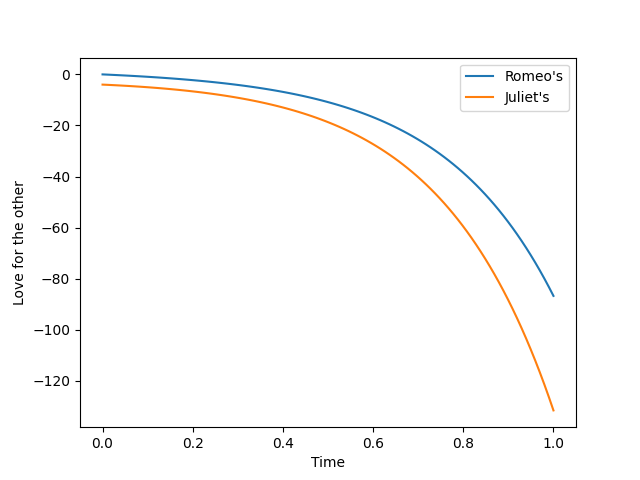
\includegraphics[width=10cm]{images/eager_beaver_1.png}
    \end{center}
    \caption{The love between two eager beaver}
\end{figure}\\
Giải thích các đoạn code trong \textit{Python} vẽ đồ thị ví dụ trên (các đoạn code này được ta định nghĩa trong file \textbf{trajectory.py} và sẽ được dùng để vẽ \textbf{phase portrait}) như sau:
\begin{itemize}
    \item Nạp các modules cần thiết, bao gồm: \textbf{numpy} (module toán học xử lý ma trận và mảng), \textbf{matplotlib.pyplot}(module đồ họa vẽ đồ thị), \textbf{math} và khai báo ma trận hệ số (hình 2).
    \begin{figure}[h!]
        \begin{center}
        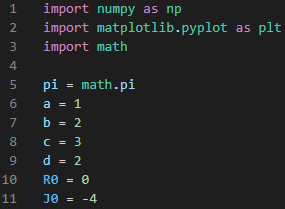
\includegraphics[width=5cm]{images/module_param.png}
        \end{center}
        \caption{Modules và khai báo}
    \end{figure}
    \item Viết hàm tính $\Delta$ và $\lambda$ (hình 3).
    \begin{figure}[h!]
        \begin{center}
        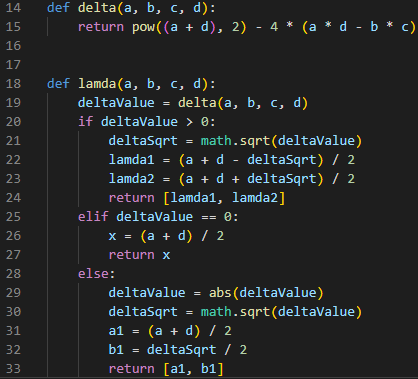
\includegraphics[width=8cm]{images/delta_lambda.png}
        \end{center}
        \caption{$\Delta$ và $\lambda$}
    \end{figure}
    \item Viết các hàm phụ tính các hằng số trong công thức tương ứng với 3 trường hợp (hình 4).
    \begin{figure}[h!]
        \begin{center}
        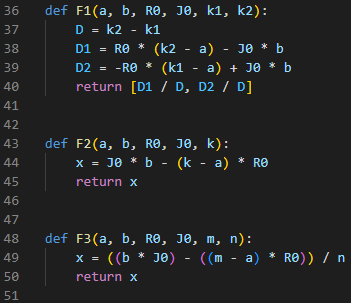
\includegraphics[width=6cm]{images/helper_func.png}
        \end{center}
        \caption{Các hàm phụ trợ tính hệ số}
    \end{figure}
    \item Hàm tính giá trị của $R$ (hình 5).
    \begin{figure}[h!]
        \begin{center}
        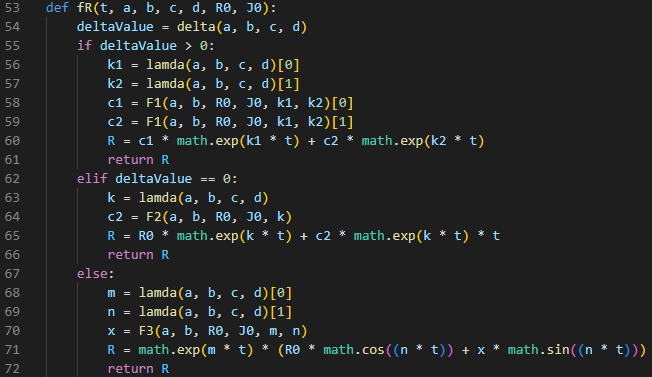
\includegraphics[width=10cm]{images/R.png}
        \end{center}
        \caption{Hàm tính giá trị $R$ theo $t$}
    \end{figure}
    \item Hàm tính giá trị của $J$ (hình 6).
    \begin{figure}[h!]
        \begin{center}
        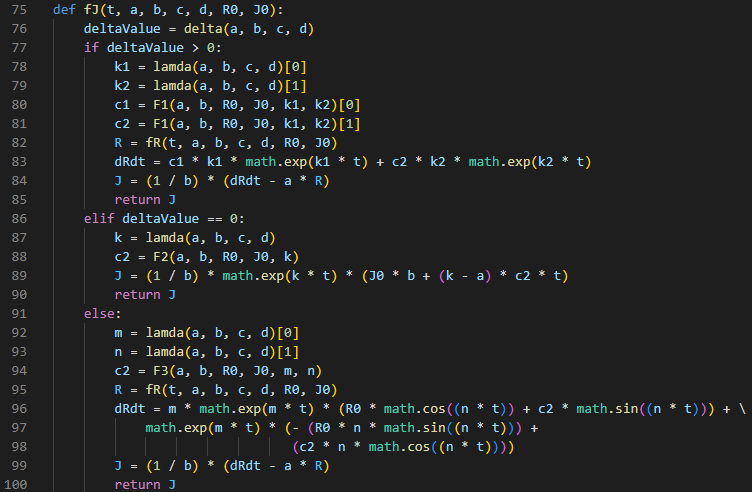
\includegraphics[width=10cm]{images/J.png}
        \end{center}
        \caption{Hàm tính giá trị $J$ theo $t$}
    \end{figure}
    \item Lấy 100 giá trị của biến thời gian $t$ trong khoảng $[0,1]$ để vẽ đồ thị (hình 7).
    \begin{figure}[h!]
        \begin{center}
        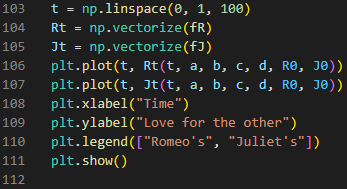
\includegraphics[width=5cm]{images/trajectory.png}
        \end{center}
        \caption{Vẽ đồ thị}
    \end{figure}
\end{itemize}
\subsubsection{Ví dụ 2}
\begin{align*}
    \begin{cases}
        R'=R+2J\\
        J'=3R+2J\\
        R(0)=1\\
        J(0)=2
    \end{cases}
\end{align*}
Tương tự ví dụ 1 nhưng $R_0=1, J_0=2$
Áp dụng công thức nghiệm chính xác ở trường hợp 1:
\begin{align*}
    \begin{cases}
        R(t)=-\frac{1}{5}e^{-t}+\frac{6}{5}e^{4t}\\
        J(t)=\frac{1}{5}e^{-t}+\frac{9}{5}e^{4t}
    \end{cases}
\end{align*}
Đồ thi biểu diễn như sau (hình 8):
\begin{figure}[h!]
    \begin{center}
    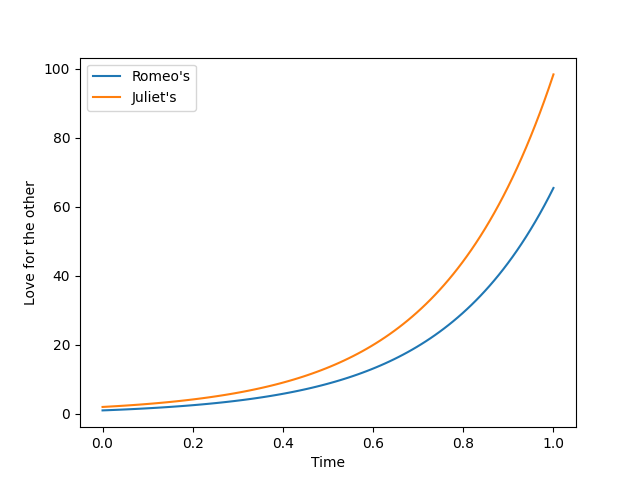
\includegraphics[width=10cm]{images/eager_beaver_2.png}
    \end{center}
    \caption{The love between two eager beaver}
\end{figure}
\subsubsection{Phase portrait}
Ứng với hệ phương trình trong 2 ví dụ trên với các điều kiện ban đầu bất kì
$\begin{cases}
        R'=R+2J\\
        J'=3R+2J
\end{cases}$
ta có phase portrait trong mặt phẳng $RJ$ được biểu diễn trong hình 9
\begin{figure}[h!]
    \begin{center}
    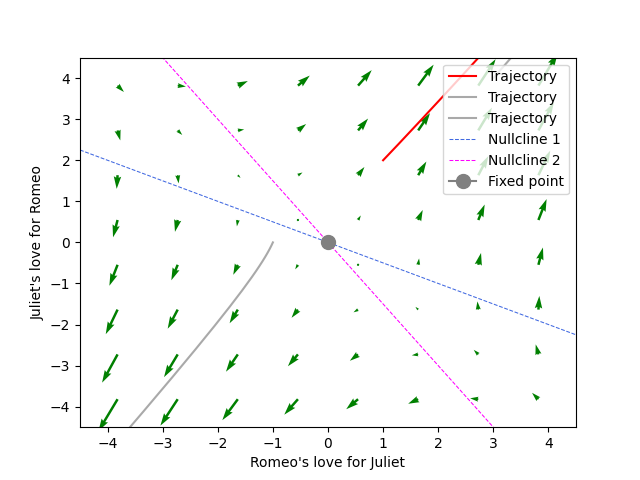
\includegraphics[width=10cm]{images/phase_portrait_eager_beaver.png}
    \end{center}
    \caption{The phase portrait of the love between two eager beaver}
\end{figure}\\
Giải thích các đoạn code trong \textit{Python} vẽ phase portrait:
\begin{itemize}
    \item Nạp các modules cần thiết, bao gồm \textbf{numpy}, \textbf{matplotlib.pyplot}, package \textbf{odeint} trong module \textbf{scipy.integrate} (dùng để giải hệ phương trình vi phân), các thông số $a, b, c, d, R_0, J_0$ trong module \textbf{trajectory} (module này đã được ta định nghĩa). Ta sẽ vẽ các trajectory ứng với các bộ giá trị ban đầu $[R_0, J_0], [R_0+2,J_0+2], [R_0-2,J_0-2]$ (hình 10).
    \begin{figure}[h!]
        \begin{center}
        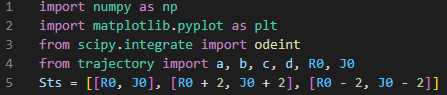
\includegraphics[width=8cm]{images/pakage_init.png}
        \end{center}
        \caption{Modules, pakage và khai báo các bộ giá trị ban đầu}
    \end{figure}
    \item Viết hàm biểu diễn hệ phương trình vi phân (hình 11).
    \begin{figure}[h!]
        \begin{center}
        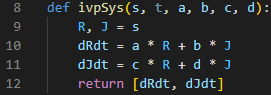
\includegraphics[width=5cm]{images/ivpSys.png}
        \end{center}
        \caption{Hàm biểu diễn hệ phương trình vi phân}
    \end{figure}
    \item Vẽ các vector biểu diễn $R'$ và $J'$ tại thời điểm ban đầu $t=0$ của một tập gồm 144 điểm rời rạc $(R_0,J_0)$ phân bố đều nhau trên mặt phẳng $RJ$ (hình 12).
    \begin{figure}[h!]
        \begin{center}
        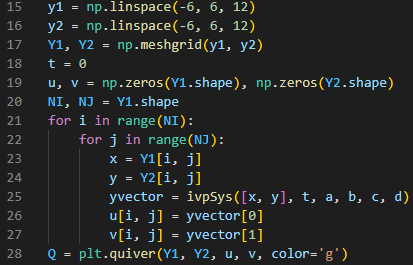
\includegraphics[width=8cm]{images/vector_field.png}
        \end{center}
        \caption{Vẽ các vector biểu diễn $R'$ và $J'$}
    \end{figure}
    \item Vẽ các trajectory với 200 giá trị của biến thời gian $t$ từ $(0, 5)$ ứng với 3 bộ giá trị ban đầu: $(R_0, J_0)$ (màu đỏ) và $(R_0 + 2, J_0 + 2), (R_0 - 2, J_0 - 2)$ (màu xám) (hình 13).
    \begin{figure}[h!]
        \begin{center}
        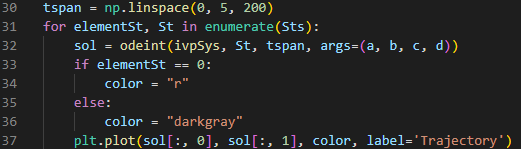
\includegraphics[width=10cm]{images/plot_odeint.png}
        \end{center}
        \caption{Vẽ các trajectory}
    \end{figure}
    \item Ký hiệu các chú thích và vẽ phase portrait (hình 14).
    \begin{figure}[h!]
        \begin{center}
        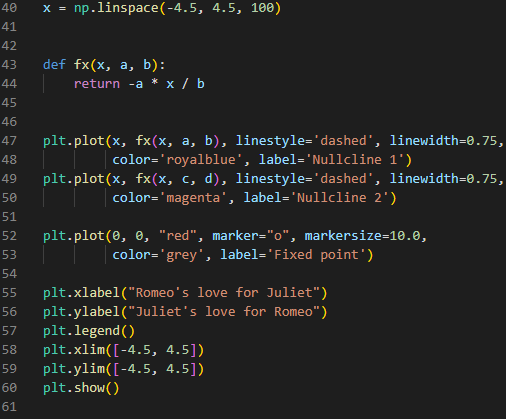
\includegraphics[width=10cm]{images/phase_portrait.png}
        \end{center}
        \caption{Vẽ phase portrait}
    \end{figure}
\end{itemize}
\subsection{Narcissistic Nerd}
Điều kiện của a, b trong phong cách này là $a > 0$ và $b < 0$. Ta xét 2 ví dụ cùng ma trận hệ số nhưng điều kiện ban đầu khác nhau. Đoạn code trong \textit{Python} dùng để vẽ các đồ thị và phase portrait tương tự mục Eager Beaver, chỉ thay đổi tham số $a, b, c, d, R_0, J_0$.
\subsubsection{Ví dụ 1}
\begin{align*}
    \begin{cases}
        R'=5R-J\\
        J'=R+3J\\
        R(0)=1\\
        J(0)=2
    \end{cases}
\end{align*}
Theo bài 1, ta có $\Delta=0$, hệ có 1 trị riêng duy nhất $\lambda=4$. Áp dụng công thức nghiệm chính xác ở trường hợp 3:
\begin{align*}
    \begin{cases}
        R(t)=e^{4t}(-t+1)\\
        J(t)=e^{4t}(-t+2)
    \end{cases}
\end{align*}
Biểu diễn $R$ (narcissistic nerd) và $J$ (eager beaver) trên cùng một đồ thị theo biến thời gian $t$ (hình 15):
\begin{figure}[h!]
    \begin{center}
    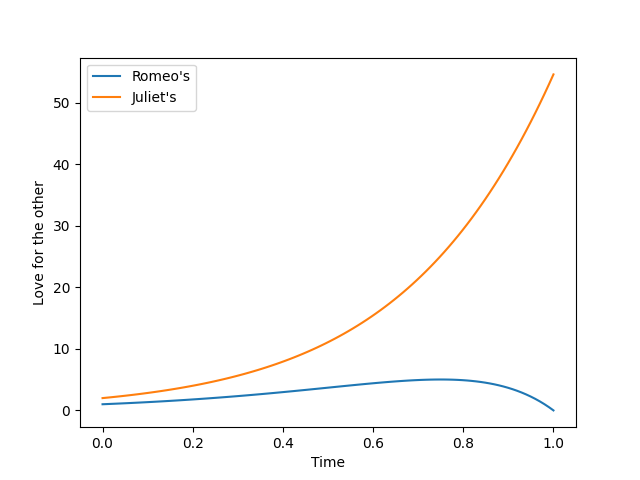
\includegraphics[width=10cm]{images/narcissistic_nerd_1.png}
    \end{center}
    \caption{The love between a narcissistic nerd and a eager beaver}
\end{figure}
\subsubsection{Ví dụ 2}
\begin{align*}
    \begin{cases}
        R'=5R-J\\
        J'=R+3J\\
        R(0)=1\\
        J(0)=3
    \end{cases}
\end{align*}
Tương tự ví dụ 1 nhưng $R_0 = 1, J_0 = 3$ Áp dụng công thức nghiệm chính xác ở trường hợp 3:
\begin{align*}
    \begin{cases}
        R(t)=e^{4t}(-2t+1)\\
        J(t)=e^{4t}(-2t+3)
    \end{cases}
\end{align*}
Đồ thị biểu diễn ở hình 16.
\begin{figure}[h!]
    \begin{center}
    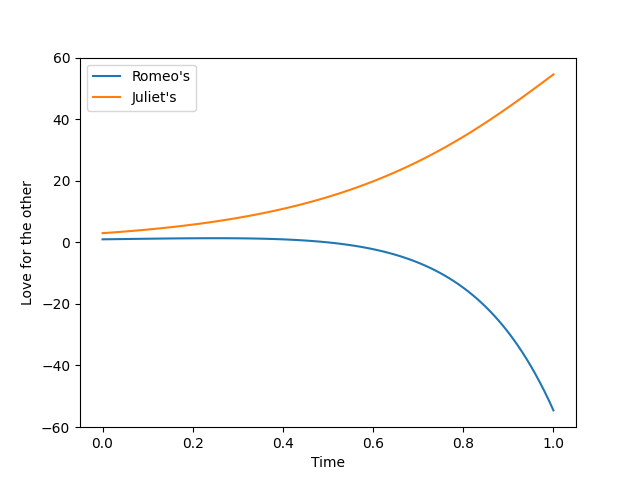
\includegraphics[width=10cm]{images/narcissistic_nerd_2.png}
    \end{center}
    \caption{The love between a narcissistic nerd and a eager beaver}
\end{figure}
\subsubsection{Phase portrait}
Ứng với hệ phương trình trong 2 ví dụ trên với các điều kiện ban đầu bất kì
$\begin{cases}
        R'=5R-J\\
        J'=R+3J
\end{cases}$
ta có phase portrait trong mặt phẳng $RJ$ được biểu diễn trong hình 17.
\begin{figure}[h!]
    \begin{center}
    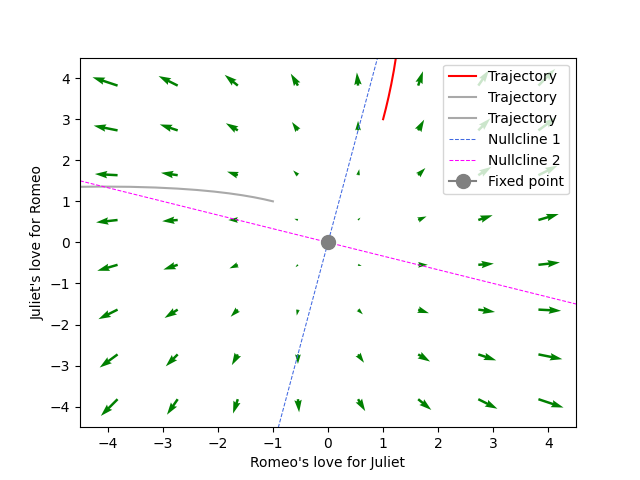
\includegraphics[width=10cm]{images/phase_portrait_narcissistic_nerd.png}
    \end{center}
    \caption{The phase portrait of the love between a narcissistic nerd and a eager beaver}
\end{figure}
\subsection{Cautious Lover}
Điều kiện của a, b trong phong cách này là $a < 0$ và $b > 0$. Ta xét 2 ví dụ cùng ma trận hệ số nhưng điều kiện ban đầu khác nhau. Đoạn code trong \textit{Python} dùng để vẽ các đồ thị và phase portrait tương tự mục Eager Beaver, chỉ thay đổi tham số $a, b, c, d, R_0, J_0$.
\subsubsection{Ví dụ 1}
\begin{align*}
    \begin{cases}
        R'=-3R+9J\\
        J'=-2R+3J\\
        R(0)=1\\
        J(0)=2
    \end{cases}
\end{align*}
Theo bài 1, ta có $\Delta=-36<0$, hệ có 2 trị riêng phức liên hợp $\lambda_{1,2}= \pm 3i$. Áp dụng công thức nghiệm chính xác ở trường hợp 2:
\begin{align*}
    \begin{cases}
        R(t)=\cos{3t}+5\sin{3t}\\
        J(t)=2\cos{3t}+\frac{4}{3}\sin{3t}
    \end{cases}
\end{align*}
Biểu diễn $R$ (cautious lover) và $J$ (narcissistic nerd) trên cùng một đồ thị theo biến thời gian $t$ (hình 18):
\begin{figure}[h!]
    \begin{center}
    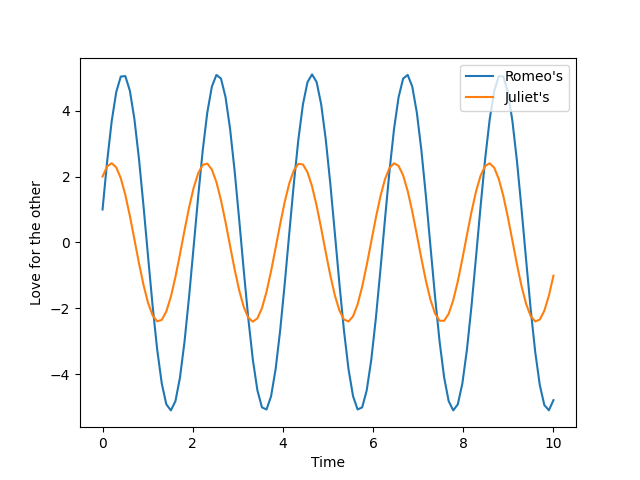
\includegraphics[width=10cm]{images/cautious_lover_1.png}
    \end{center}
    \caption{The love between a cautious lover and a narcissistic nerd}
\end{figure}
\subsubsection{Ví dụ 2}
\begin{align*}
    \begin{cases}
        R'=-3R+9J\\
        J'=-2R+3J\\
        R(0)=2\\
        J(0)=-4
    \end{cases}
\end{align*}
Tương tự ví dụ 1 nhưng $R_0 = 2, J_0 = -4$ Áp dụng công thức nghiệm chính xác ở trường hợp 2:
\begin{align*}
    \begin{cases}
        R(t)=2\cos{3t}-14\sin{3t}\\
        J(t)=-4\cos{3t}-\frac{16}{3}\sin{3t}
    \end{cases}
\end{align*}
Đồ thị biểu diễn ở hình 19.
\begin{figure}[h!]
    \begin{center}
    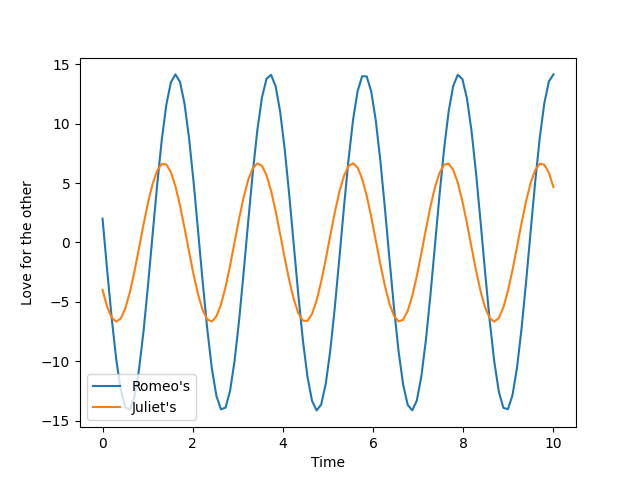
\includegraphics[width=10cm]{images/cautious_lover_2.png}
    \end{center}
    \caption{The love between a cautious lover and a narcissistic nerd}
\end{figure}
\subsubsection{Phase portrait}
Ứng với hệ phương trình trong 2 ví dụ trên với các điều kiện ban đầu bất kì
$\begin{cases}
        R'=-3R+9J\\
        J'=-2R+3J
\end{cases}$
ta có phase portrait trong mặt phẳng $RJ$ được biểu diễn trong hình 20.
\begin{figure}[h!]
    \begin{center}
    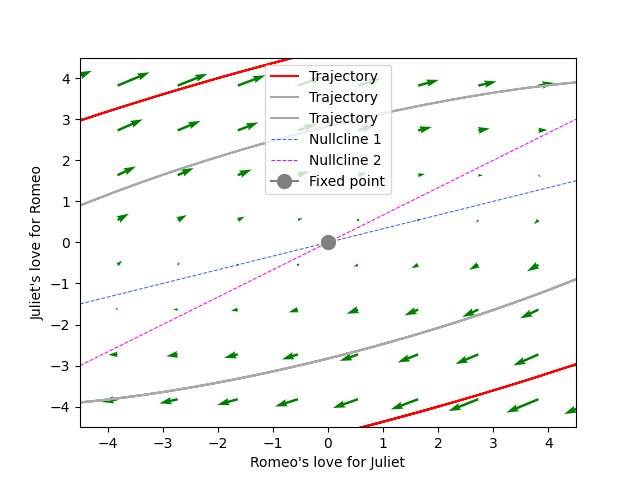
\includegraphics[width=10cm]{images/phase_portrait_cautious_lover.png}
    \end{center}
    \caption{The phase portrait of the love between a cautious lover and a narcissistic nerd}
\end{figure}
\subsection{Hermit}
Điều kiện của a, b trong phong cách này là $a < 0$ và $b < 0$. Ta xét 2 ví dụ cùng ma trận hệ số nhưng điều kiện ban đầu khác nhau. Đoạn code trong \textit{Python} dùng để vẽ các đồ thị và phase portrait tương tự mục Eager Beaver, chỉ thay đổi tham số $a, b, c, d, R_0, J_0$.
\subsubsection{Ví dụ 1}
\begin{align*}
    \begin{cases}
        R'=-3R-13J\\
        J'=5R-J\\
        R(0)=3\\
        J(0)=1
    \end{cases}
\end{align*}
Theo bài 1, ta có $\Delta=-256<0$, hệ có 2 trị riêng phức liên hợp $\lambda_{1,2}=-2\pm8i$. Áp dụng công thức nghiệm chính xác ở trường hợp 2:
\begin{align*}
    \begin{cases}
        R(t)=e^{-2t}(3\cos{8t}-2\sin{8t})\\
        J(t)=e^{-2t}(\cos{8t}+2\sin{8t})
    \end{cases}
\end{align*}
Biểu diễn $R$ (hermit) và $J$ (cautious lover) trên cùng một đồ thị theo biến thời gian $t$ (hình 21):
\begin{figure}[h!]
    \begin{center}
    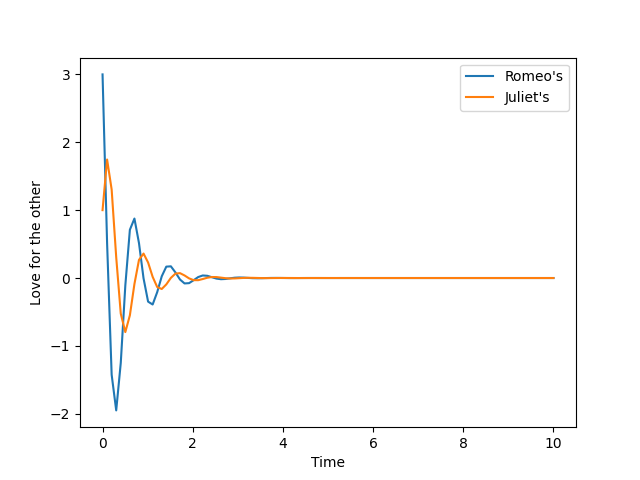
\includegraphics[width=10cm]{images/hermit_1.png}
    \end{center}
    \caption{The love between a hermit and a cautious lover}
\end{figure}
\subsubsection{Ví dụ 2}
\begin{align*}
    \begin{cases}
        R'=-3R-13J\\
        J'=5R-J\\
        R(0)=2\\
        J(0)=-2
    \end{cases}
\end{align*}
Tương tự ví dụ 1 nhưng $R_0 = 2, J_0 = -2$ Áp dụng công thức nghiệm chính xác ở trường hợp 2:
\begin{align*}
    \begin{cases}
        R(t)=e^{-2t}(2\cos{8t}+3\sin{8t})\\
        J(t)=e^{-2t}(-2\cos{8t}+\sin{8t})
    \end{cases}
\end{align*}
Đồ thị biểu diễn ở hình 22.
\begin{figure}[h!]
    \begin{center}
    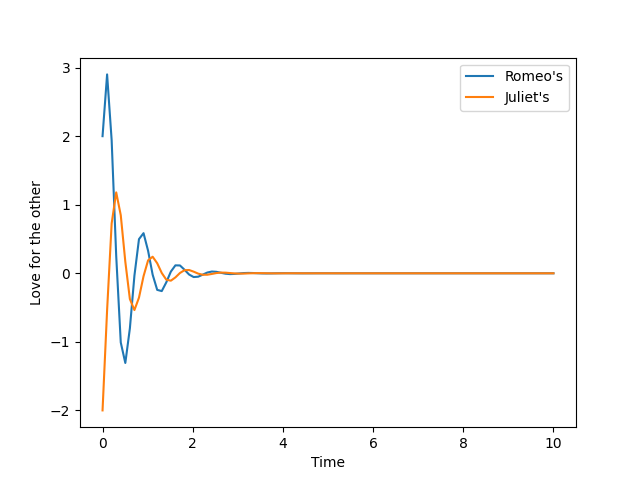
\includegraphics[width=8cm]{images/hermit_2.png}
    \end{center}
    \caption{The love between a hermit and a cautious lover}
\end{figure}
\subsubsection{Phase portrait}
Ứng với hệ phương trình trong 2 ví dụ trên với các điều kiện ban đầu bất kì
$\begin{cases}
        R'=-3R-13J\\
        J'=5R-J
\end{cases}$
ta có phase portrait trong mặt phẳng $RJ$ được biểu diễn trong hình 23.
\begin{figure}[h!]
    \begin{center}
    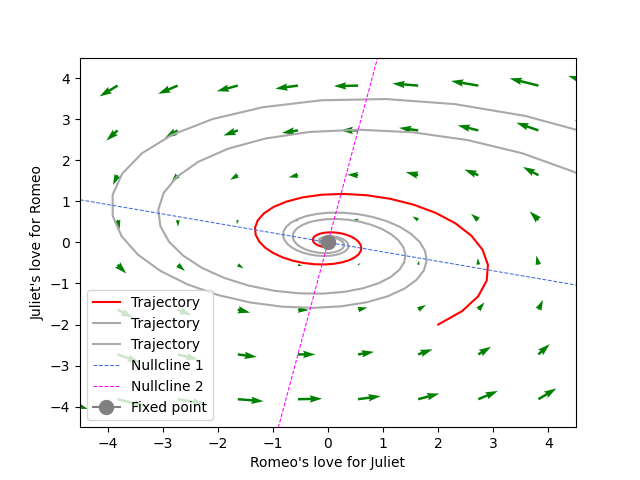
\includegraphics[width=9cm]{images/phase_portrait_hermit.png}
    \end{center}
    \caption{The phase portrait of the love between a hermit and a cautious lover}
\end{figure}
\newpage
\section{Bài tập 3}
\subsection{Hệ phương trình vi phân tuyến tính không thuần nhất với hệ số hằng (Nonhomogeneous Linear System)}
Khi tình yêu giữa Romeo và Juliet phụ thuộc vào điều kiện bên ngoài (như gia đình, xã hội,..) ta sẽ có hệ phương trình tổng quát như sau:
\begin{align}
    \begin{cases}
        R'=aR+bJ+f(t)\\
        J'=cR+dJ+g(t)\\
        R(0)=R_0, J(0)=J_0
    \end{cases}
\end{align}
Trong đó:\\
$R:\mathbb{R^+}\cup\{0\}\to \mathbb{R}$ (\textit{hàm đại diện tình yêu của Romeo dành cho Juliet)}.\\
$J:\mathbb{R^+}\cup\{0\}\to \mathbb{R}$(\textit{hàm đại diện tình yêu của Juliet dành cho Romeo)}.\\
$a$, $b$, $c$, $d$ $\in\mathbb{R}$: mô tả sự tương tác tình yêu của một người đến người còn lại.\\
$R_0$, $J_0$: lần lượt là tình yêu của Romeo dành cho Juliet và của Juliet dành cho Romeo tại thời điểm ban đầu.\\
$f(t)$, $g(t)$ là hai hàm theo biến thời gian $t$, lần lượt là điều kiện bên ngoài ảnh hưởng tới tình yêu của Romeo và Juliet.\\\\
Hệ (15) có dạng hệ phương trình vi phân tuyến tính không thuần nhất. Ta biểu diễn lại hệ (15) dưới dạng tổng quát:\\
\begin{align}
    \begin{cases}
        x'=Ax+B(t)\\
        x(0)=x_0
    \end{cases}
\end{align}
Để tìm nghiệm tổng quát cho hệ (15), ta sẽ tìm cách giải và nghiệm tổng quát của hệ (16).\\
\subsubsection{Hàm mũ ma trận (Matrix Exponential)}
\subsubsubsection{Định nghĩa}
Cho $A$ là một ma trận $n \times n$ với hệ số không đổi. Hàm mũ ma trận của $A$ (kí hiệu là $e^{At}$) được biểu diễn như sau:\\
$$e^{At}=\sum_{k=0}^{\infty}A^{k}\frac{t^{k}}{k!}=I_n+At+\frac{1}{2!}A^{2}t^{2}+\frac{1}{3!}A^{3}t^{3}+...$$
\subsubsubsection{Áp dụng hàm mũ ma trận trong tìm nghiệm hệ phương trình vi phân trình vi phân tuyến tính thuần nhất}
Cho hệ phương trình vi phân tuyến tính thuần nhất:
\begin{align}
    \begin{cases}
        x'=Ax\\
        x(0)=x_0
    \end{cases}
\end{align}
Giả sử $e^{At}$ là hàm mũ ma trận của $A$, ta được nghiệm tổng quát của hệ (17):
\begin{align}
    x=e^{At}x_0
\end{align}
\textbf{Thật vậy, ta có thể chứng minh công thức trên như sau:}\\
Dựa và định nghĩa ta có:\\
$$e^{At}=I_n+At+\frac{1}{2!}A^{2}t^{2}+\frac{1}{3!}A^{3}t^{3}+...$$
$$\Rightarrow\frac{d}{dt}(e^{At})=A+A^{2}t+\frac{1}{2}A^{3}t^{2}+...$$
$$\Rightarrow\frac{d}{dt}(e^{At})=A(I_n+At+\frac{1}{2}A^{2}t^{2}+...)$$
$$\Rightarrow\frac{d}{dt}(e^{At})=Ae^{At}$$
Điều này cho thấy $e^{At}$ là nghiệm của hệ phương trình vi phân tuyến tính $x'=Ax$. Nghiệm $x$ lúc này được biểu diễn dưới dạng $x=e^{At}.c$ (với c là hằng số). 
Kết hợp với điều kiện ban đầu $x(0)=x_0$, ta được nghiệm tổng quát của hệ (17):
\begin{align*}
    x=e^{At}x_0
\end{align*}
\subsubsubsection{Phương pháp tìm hàm mũ ma trận}
Như ta chứng minh ở trên, nếu có hàm mũ của ma trận A thì ta sẽ tìm được nghiệm của hệ phương trình vi phân tuyến tính thuần nhất. Nhưng làm cách nào để tìm được hàm mũ của một ma trận? Sau đây sẽ là một số phương pháp được sử dụng để tìm hàm mũ ma trận.
\subsubsubsection*{Phương pháp sử dụng định nghĩa}
Với phương pháp này, ta chỉ áp dụng với các ma trận khi lũy thừa có điểm dừng hoặc có thể đưa về dạng tổng quát.\\
Ta xét các ví dụ sau:
\subsubsubsection*{Ví dụ 1}
Tìm hàm mũ của ma trận $A=
\begin{bmatrix}
0 & 1\\
0 & 0
\end{bmatrix}$\\
\textbf{Cách giải}\\
Ta tính lũy thừa liên tiếp của A:\\
$$A=
\begin{bmatrix}
0 & 1\\
0 & 0
\end{bmatrix}$$
$$A^{2}=A^{3}=...=
\begin{bmatrix}
0 & 0\\
0 & 0
\end{bmatrix}$$
$$\Rightarrow e^{At}=I_n+At=
\begin{bmatrix}
1 & t\\
0 & 1
\end{bmatrix}$$
\subsubsubsection*{Ví dụ 2}
Tìm hàm mũ của ma trận $A=
\begin{bmatrix}
2 & 0\\
0 & 3
\end{bmatrix}$\\
\textbf{Cách giải}\\
Ta tính lũy thừa liên tiếp của A:\\
$$A=
\begin{bmatrix}
2 & 0\\
0 & 3
\end{bmatrix}$$
$$A^{2}=
\begin{bmatrix}
4 & 0\\
0 & 9
\end{bmatrix}$$
$$\vdots\\$$
$$A^{n}=
\begin{bmatrix}
2^{n} & 0\\
0 & 3^{n}
\end{bmatrix}$$
$$\Rightarrow e^{At}=\sum_{k=0}^{\infty}\frac{t^{k}}{k!}\begin{bmatrix}
2^{n} & 0\\
0 & 3^{n}
\end{bmatrix}$$
\textbf{Nhận xét:}\\
Nếu tính lũy thừa của A như trong hai ví dụ trên, ta sẽ rất khó khi tính những hàm mũ không có quy luật rõ ràng. Vì vậy ta sẽ tìm hiểu thêm những phương pháp tiếp theo.
\subsubsubsection*{Phương pháp dùng đại số tuyến tính}
Phương pháp này được áp dụng khi ma trận cần tìm hàm mũ là một ma trận chéo hóa được.\\
Cho $A$ là một ma trận $n \times n$ với hệ số không đổi. Giả sử ma trận $A$ chéo hóa được với các vectơ riêng độc lập $v_1, v_2,...,v_n$ và các trị riêng tương ứng $\lambda_1,\lambda_2,...,\lambda_n$.\\
Đặt:
$$S=
\begin{bmatrix}
    v_1 & v_2 &.. &v_n
\end{bmatrix}$$
$$D=
\begin{bmatrix}
    \lambda_1 & 0 &... &0\\
    0 & \lambda_2 &... &0\\
    \vdots & \vdots&\vdots& \vdots\\
    0 & 0 &.. &\lambda_n\\
\end{bmatrix}$$
$$\Rightarrow S^{-1}.A.S=D$$
Khi đó:
$$e^{Dt}=
\begin{bmatrix}
    e^{\lambda_1t} & 0 &... &0\\
    0 & e^{\lambda_2t} &... &0\\
    \vdots & \vdots&\vdots& \vdots\\
    0 & 0 &.. &e^{\lambda_nt}\\
\end{bmatrix}$$
Ta lại có:
$$e^{Dt}=\sum_{n=0}^{\infty}\frac{t^{n}(S^{-1}AS)^{n}}{n!}=\sum_{n=0}^{\infty}\frac{t^{n}S^{-1}A^{n}S}{n!}=S^{-1}\sum_{n=0}^{\infty}\frac{t^{n}A^{n}}{n!}S=S^{-1}e^{At}S$$
Suy ra:
$$e^{At}=Se^{Dt}S^{-1}$$
Hay
\begin{align}
    e^{At}=S
\begin{bmatrix}
    e^{\lambda_1t} & 0 &... &0\\
    0 & e^{\lambda_2t} &... &0\\
    \vdots & \vdots&\vdots& \vdots\\
    0 & 0 &.. &e^{\lambda_nt}\\
\end{bmatrix}
S^{-1}
\end{align}
\subsubsubsection*{Phương pháp Williamson}
Phương pháp này được áp dụng khi ma trận cần tìm hàm mũ không chéo hóa được.\\\\
Cho $A$ là một ma trận $n \times n$ với hệ số không đổi. Giả sử ${\lambda_1,\lambda_2,...,\lambda_n}$ là danh sách các trị riêng, với nhiều giá trị lặp lại theo bội số của chúng.\\
Đặt:
$$\begin{cases}
        a_1=e^{\lambda_1t}\\
        a_k=\displaystyle\int\limits_{0}^{t} \mathrm{e}^{\lambda_k(t-u)}a_{k-1}(u)\mathrm{d}u
\end{cases}$$
$$\begin{cases}
        B_1=I\\
        B_2=(A-\lambda_{k-1}I)B_{k-1}
\end{cases}$$
Với $k=2, 3,..., n$\\
Khi đó, ta có hàm mũ ma trận:
\begin{align}
   e^{At}=a_1B_1+a_2B_2+...+a_nB_n
\end{align}
\subsubsection{Các tính chất về nghiệm hệ phương trình vi phân tuyến tính không thuần nhất với hệ số hằng}
\textbf{Định lí 1:} Nếu $X^*(t)$ là nghiệm của hệ phương trình vi phân tuyến tính không thuần nhất với hệ số hằng, $X_1(t), X_2(t),...,X_n(t)$ là hệ nghiệm cơ bản của hệ phương trình vi phân tuyến tính thuần nhất với hệ số hằng tương ứng thì nghiệm tổng quát của hệ phương trình vi phân tuyến tính không thuần nhất với hệ số hằng có dạng:
$$X=c_1X_1(t)+c_2X_2(t)+...+C_nX_n(t)+X^*(t)$$
trong đó $c_1,c_2,...,c_n$ là các hằng số bất kì.\\\\
\textbf{Định lí 2:} Nếu $X_1(t), X_2(t)$ là hai nghiệm tương ứng của các hệ phương trình
$$x'=Ax+F_1(x); \hspace{1cm}x'=Ax+F_2(x)$$
thì $X(t)=X_1(t)+X_2(t)$ là nghiệm của hệ phương trình
$$x'=Ax+F_1(x)+F_2(x)$$
\subsubsection{Nghiệm tổng quát của hệ phương trình vi phân tuyến tính không thuần nhất với hệ số hằng}
Trở lại với hệ $(16)$:
\begin{align*}
    \begin{cases}
        x'=Ax+B(t)\\
        x(0)=x_0
    \end{cases}
\end{align*}
Gọi $x_c$ là nghiệm của hệ phương trình thuần nhất:
\begin{align*}
    \begin{cases}
        x'=Ax\\
        x(0)=x_0
    \end{cases}
\end{align*}
Gọi $x_p$ là nghiệm riêng của hệ $(16$).\\
\textbf{Ta được nghiệm tổng quát của hệ $(16)$ có dạng như sau:}
\begin{align*}
    x=x_c+x_p
\end{align*}
Ta tiếp tục tìm dạng tổng quát của $x_c$ và $x_p$\\
Dựa và công thức $(18)$ nghiệm $x_c$ có dạng:
\begin{align*}
    x_c=e^{At}x_0
\end{align*}
Suy ra, nghiệm $x_p$ có dạng:
\begin{align*}
    x_p=e^{At}U(t)
\end{align*}
Ta tiếp tục tìm dạng tổng quát của U(t).\\
Thay $x_p$ vào hệ $(16)$ ta được:
$$x_p'=Ax_p+B(t)$$
$$\Rightarrow Ae^{At}U(t)+e^{At}U'(t)=Ae^{At}U(t)+B(t)$$
$$\Rightarrow e^{At}U'(t)=B(t)$$
$$U(t)=\displaystyle\int\limits_{0}^{t} \mathrm{e}^{-As}B(s)\mathrm{d}s$$
\textbf{Suy ra, nghiệm của hệ $(16)$ có dạng tổng quát:}
\begin{align}
    x=e^{At}x_0+\displaystyle\int\limits_{0}^{t} \mathrm{e}^{A(t-s)}B(s)\mathrm{d}s
\end{align}
\subsubsubsection*{Từ công thức nghiệm $(21)$, ta suy ra hệ $(15)$ có nghiệm như sau:}
\begin{align}
\begin{bmatrix}
    R\\
    J
\end{bmatrix}
    =e^{At}x_0+\displaystyle\int\limits_{0}^{t} \mathrm{e}^{A(t-s)}
\begin{bmatrix}
    f(x)\\
    g(x)
\end{bmatrix}
    \mathrm{d}s
\end{align}
\subsubsection{Ví dụ tìm nghiệm của hệ phương trình vi phân tuyến tính không thuần nhất với hệ số không đổi}
\textbf{Ví dụ 1:} Tìm nghiệm của hệ phương trình sau:
\begin{align*}
    \begin{cases}
        R'=-3R+4J+sin(t)\\
        J'=-2R+3J+t\\
        R(0)=0, J(0)=1
    \end{cases}
\end{align*}
\centerline{\textbf{Giải}}
Biểu diễn hệ phương trình trên lại dưới dạng:
\begin{align*}
    \begin{cases}
        x'=
        \begin{bmatrix}
        -3 & 4\\
        -2 & 3
        \end{bmatrix}
        x+
        \begin{bmatrix}
        sin(t)\\
        t
        \end{bmatrix}\\
        x(0)=\begin{bmatrix}
        0\\
        1
        \end{bmatrix}
    \end{cases}
\end{align*}
\hspace{0.3cm}Với $x=
\begin{bmatrix}
    R\\
    J
\end{bmatrix}$\\
Xét ma trận $A=
\begin{bmatrix}
    -3&4\\
    -2&3
\end{bmatrix}
$\\
Phương trình đặc trưng của A có 2 trị riêng thực phân biệt $\lambda_1=1; \lambda_2=-1$, vectơ riêng tương ứng là $v_1=
\begin{bmatrix}
    1\\
    1
\end{bmatrix};
v_2=
\begin{bmatrix}
    2\\
    1
\end{bmatrix}
$.
Suy ra hàm mũ của A:\\
\hspace*{4cm}$e^{At}=
\begin{bmatrix}
    1 &2\\
    1 & 1
\end{bmatrix}
\begin{bmatrix}
    e^t & 0\\
    0 & e^{-t}
\end{bmatrix}
\begin{bmatrix}
    1 &2\\
    1 & 1
\end{bmatrix}^{-1}
$\\\\\\
\hspace*{4.7cm}$=
\begin{bmatrix}
    -e^t+2e^{-t} & 2e^t-2e^{-t}\\
    -e^t+e^{-t} & 2e^t-e^{-t}
\end{bmatrix}
$\\
Gọi $x_c$ là nghiệm của hệ thuần nhất suy ra từ hệ ban đầu, $x_p$ là nghiệm riêng của hệ ban đầu.\\
Suy ra:\\
\begin{align*}
x_c=e^{At}x_0=
    \begin{bmatrix}
    -e^t+2e^{-t} & 2e^t-2e^{-t}\\
    -t & 2e^t-e^{-t}
\end{bmatrix}
\begin{bmatrix}
    0\\
    1
\end{bmatrix}
=\begin{bmatrix}
    2e^t-2e^{-t}\\
    2e^t-e^{-t}
\end{bmatrix}
\end{align*}
\begin{align*}
    x_p=\displaystyle\int\limits_{0}^{t} \mathrm{e}^{A(t-s)}.
    \begin{bmatrix}
    sin(s)\\
    s
\end{bmatrix}
    \mathrm{d}s
=\displaystyle\int\limits_{0}^{t}
\begin{bmatrix}
    -e^{t-s}+2e^{-(t-s)} & 2e^{t-s}-2e^{-(t-s)}\\
    -e^{t-s}+e^{-(t-s)} & 2e^{t-s}-e^{-(t-s)}
\end{bmatrix}
\begin{bmatrix}
    sin(s)\\
    s
\end{bmatrix}
\mathrm{d}s
\end{align*}
\begin{align*}
    =\begin{bmatrix}
\displaystyle\int\limits_{0}^{t}((sin(s)(-e^{t-s}+2e^{-t+s}))+s(2e^{t-s}-2e^{-t+s}))\mathrm{d}s\\
\displaystyle\int\limits_{0}^{t}((sin(s)(-e^{t-s}+e^{-t+s}))+s(2e^{t-s}-e^{-t+s}))\mathrm{d}s
\end{bmatrix}
\end{align*}
\begin{align*}
    =\begin{bmatrix}
    -4t+\frac{3}{2}e^t-e^{-t}-\frac{1}{2}cos(t)+\frac{3}{2}sin(t) \\
    -1-3t+\frac{3}{2}e^t-\frac{1}{2}e^{-t}+sin(t)
\end{bmatrix}
\end{align*}
Suy ra nghiệm của hệ phương trình ban đầu:\\
\begin{align*}
    x=x_c+x_p
=\begin{bmatrix}
    \frac{7}{2}e^t-3e^{-t}+\frac{3}{2}sin(t)-\frac{1}{2}cos(t)-4t\\
    \frac{7}{2}e^t-\frac{3}{2}e^{-t}+sin(t)-3t-1
\end{bmatrix}
\end{align*}
Vậy hệ phương trình đã cho có nghiệm duy nhất:
\begin{align*}
    R= \frac{7}{2}e^t-3e^{-t}+\frac{3}{2}sin(t)-\frac{1}{2}cos(t)-4t\\
    J= \frac{7}{2}e^t-\frac{3}{2}e^{-t}+sin(t)-3t-1
\end{align*}
\textbf{Ví dụ 2:} Tìm nghiệm của hệ phương trình sau:
\begin{align*}
    \begin{cases}
        R'=3R-J+t\\
        J'=R+J+t^2\\
        R(0)=3, J(0)=4
    \end{cases}
\end{align*}
\centerline{\textbf{Giải}}
Biểu diễn hệ phương trình trên lại dưới dạng:
\begin{align*}
    \begin{cases}
        x'=
        \begin{bmatrix}
        3 & -1\\
        1 & 1
        \end{bmatrix}
        x+
        \begin{bmatrix}
        t\\
        t^2
        \end{bmatrix}\\
        x(0)=\begin{bmatrix}
        3\\
        4
        \end{bmatrix}
    \end{cases}
\end{align*}
\hspace{0.3cm}Với $x=
\begin{bmatrix}
    R\\
    J
\end{bmatrix}$\\
Xét ma trận $A=
\begin{bmatrix}
    3&-1\\
    1&1
\end{bmatrix}.
$
 Phương trình đặc trưng $det(A- \lambda I)=0$ có nghiệm bội $\lambda_1=\lambda_2=2$.\\
Để tìm hàm mũ của ma trận A. Ta sẽ tính dãy $a_k$ và $B_k$ (với k=1,2):\\
Dãy $a_k$:
\begin{align*}
    \begin{cases}
        a_1=e^{2t}\\
        a_2=\displaystyle\int\limits_{0}^{t} \mathrm{e}^{2(t-u)}*\mathrm{e}^{2u}\mathrm{d}u=e^{2t}\displaystyle\int\limits_{0}^{t}\mathrm{d}u=t.e^{2t}
    \end{cases}
\end{align*}
Dãy $B_k$:
\begin{align*}
    \begin{cases}
        B_1=I\\
        B_2=(A-2I)I=A-2I=
        \begin{bmatrix}
            1 &-1\\
            1 &-1
        \end{bmatrix}
    \end{cases}
\end{align*}
Suy ra hàm mũ của A:
$$e^{At}=a_1.B_1+a_2.B_2=
e^{2t}
\begin{bmatrix}
    1 &0\\
    0&1
\end{bmatrix}
+ t.e^{2t}.
\begin{bmatrix}
    1&-1\\
    1&-1
\end{bmatrix}
$$
$$=
\begin{bmatrix}
    e^{2t}+t.e^{2t}&-te^{2t}\\
    te^{2t} & e^{2t}-te^{2t}
\end{bmatrix}$$
Suy ra nghiệm của hệ phương trình thuần nhất:
$$x_c=e^{At}.x_0=
\begin{bmatrix}
    -t.e^{2t}+3e^{2t}\\
    -te^{2t}+4e^{2t}
\end{bmatrix}
$$
Nghiệm riêng của hệ phương trình đã cho:
$$
    x_p=\displaystyle\int\limits_{0}^{t} \mathrm{e}^{A(t-s)}.
    \begin{bmatrix}
    s\\
    s^2
\end{bmatrix}
    \mathrm{d}s
=\displaystyle\int\limits_{0}^{t}
\begin{bmatrix}
    e^{2(t-s)}+(t-s)e^{2(t-s)} & -(t-s)e^{2(t-s)}\\
    (t-s)e^{2(t-s)} & e^{2(t-s)}-(t-s)e^{2(t-s)}
\end{bmatrix}
\begin{bmatrix}
    s\\
    s^2
\end{bmatrix}
\mathrm{d}s
$$
$$=
\begin{bmatrix}
    \frac{1}{8}(-2t^2-6t+3e^{2t}-3)\\
    \\
    \frac{3}{8}(-2t^2-2t+e^{2t}-1)
\end{bmatrix}
$$
Vậy nghiệm của phương trình đã cho là:
$$x=x_c+x_p
\begin{bmatrix}
    -t.e^{2t}+3e^{2t}+\frac{1}{8}(-2t^2-6t+3e^{2t}-3)\\
    \\
    -te^{2t}+4e^{2t}+\frac{3}{8}(-2t^2-2t+e^{2t}-1)
\end{bmatrix}
$$
\textbf{Hay:}\\
\hspace*{3cm}$R=-t.e^{2t}+3e^{2t}+\frac{1}{8}(-2t^2-6t+3e^{2t}-3)$\\\\
\hspace*{3cm}$J=-te^{2t}+4e^{2t}+\frac{3}{8}(-2t^2-2t+e^{2t}-1)$\\\\
\textbf{Ví dụ 3:} Tìm nghiệm của hệ phương trình sau:
\begin{align*}
    \begin{cases}
        R'=J+t-1\\
        J'=-R+t^2\\
        R(0)=1, J(0)=2
    \end{cases}
\end{align*}
\centerline{\textbf{Giải}}
Biểu diễn hệ phương trình trên lại dưới dạng:
\begin{align*}
    \begin{cases}
        x'=
        \begin{bmatrix}
        0 & 1\\
        -1 & 0
        \end{bmatrix}
        x+
        \begin{bmatrix}
        t-1\\
        t^2
        \end{bmatrix}\\
        x(0)=\begin{bmatrix}
        -1\\
        2
        \end{bmatrix}
    \end{cases}
\end{align*}
\hspace{0.3cm}Với $x=
\begin{bmatrix}
    R\\
    J
\end{bmatrix}$\\
Xét ma trận $A=
\begin{bmatrix}
    0&1\\
    -1&0
\end{bmatrix}.
$
 Phương trình đặc trưng $det(A- \lambda I)=0$ có nghiệm phức với phần thực bằng 0 $\lambda_1=i$; $\lambda_2=-i$.\\
Để tìm hàm mũ của ma trận A. Ta sẽ tính dãy $a_k$ và $B_k$ (với k=1,2):\\
Dãy $a_k$:
\begin{align*}
    \begin{cases}
        a_1=e^{it}\\
        a_2=\displaystyle\int\limits_{0}^{t} \mathrm{e}^{-i(t-u)}.\mathrm{e}^{iu}\mathrm{d}u=e^{-it}\displaystyle\int\limits_{0}^{t}\mathrm{e}^{2iu}\mathrm{d}u=\frac{i}{2}(e^{-it}-e^{it})
    \end{cases}
\end{align*}
Áp dụng công thức euler: $e^{ix}=cos(x)+i.sin(x)$. Ta viết lại dãy $a_k$:
\begin{align*}
    \begin{cases}
        a_1=cos(t)+i.sin(t)\\
        a_2=\frac{i}{2}(cos(t)-i.sin(t)-cos(t)-i.sin(t))=sin(t)
    \end{cases}
\end{align*}
Dãy $B_k$:
\begin{align*}
    \begin{cases}
        B_1=I\\
        B_2=(A-iI)I=A-iI=
        \begin{bmatrix}
            -i & 1\\
            -1 & -i
        \end{bmatrix}
    \end{cases}
\end{align*}
Suy ra hàm mũ của A:
$$e^{At}=a_1.B_1+a_2.B_2=
\begin{bmatrix}
    cos(t) & sin(t)\\
    -sin(t) & cos(t)
\end{bmatrix}
$$
Suy ra nghiệm của hệ phương trình thuần nhất:
$$x_c=e^{At}.x_0=
\begin{bmatrix}
    2sin(t)-cos(t)\\
    sin(t)+2cos(t)
\end{bmatrix}
$$
Nghiệm riêng của hệ phương trình đã cho:
$$
    x_p=\displaystyle\int\limits_{0}^{t} \mathrm{e}^{A(t-s)}.
    \begin{bmatrix}
    s-1\\
    s^2
\end{bmatrix}
    \mathrm{d}s
=\displaystyle\int\limits_{0}^{t}
\begin{bmatrix}
    cos(t-s) & sin(t-s)\\
    -sin(t-s) & cos(t-s)
\end{bmatrix}
\begin{bmatrix}
    s-1\\
    s^2
\end{bmatrix}
\mathrm{d}s
$$
$$=
\begin{bmatrix}
    t^2-sin(t)+cos(t)-1\\
    t-sin(t)-cos(t)+1
\end{bmatrix}
$$
Suy ra nghiệm duy nhất của hệ phương trình đã cho:
$$x=x_p+x_c=
\begin{bmatrix}
    sin(t)+t^2-1\\
    cos(t)+t+1
\end{bmatrix}
$$
\textbf{Hay:}\\
\hspace*{5cm}$R=sin(t)+t^2-1$\\\\
\hspace*{5cm}$J=cos(t)+t+1$\\\\
\textbf{Ví dụ 4:} Tìm nghiệm của hệ phương trình sau:
\begin{align*}
    \begin{cases}
        R'=2R - 5J + e^{2t}\\
        J'=2R - 4J + e^t\\
        R(0)=1, J(0)=0
    \end{cases}
\end{align*}
\centerline{\textbf{Giải}}
Biểu diễn hệ phương trình trên lại dưới dạng:
\begin{align*}
    \begin{cases}
        x'=
        \begin{bmatrix}
        2 & -5\\
        2 & -4
        \end{bmatrix}
        x+
        \begin{bmatrix}
        e^{2t}\\
        e^t
        \end{bmatrix}\\
        x(0)=\begin{bmatrix}
        1\\
        0
        \end{bmatrix}
    \end{cases}
\end{align*}
\hspace{0.3cm}Với $x=
\begin{bmatrix}
    R\\
    J
\end{bmatrix}$\\
Xét ma trận $A=
\begin{bmatrix}
    2&-5\\
    2&-4
\end{bmatrix}.
$
 Phương trình đặc trưng $det(A- \lambda I)=0$ có nghiệm phức với phần thực khác 0 $\lambda_1=-1+i$; $\lambda_2=-1-i$.\\
Để tìm hàm mũ của ma trận A. Ta sẽ tính dãy $a_k$ và $B_k$ (với k=1,2):\\
Dãy $a_k$:
\begin{align*}
    \begin{cases}
        a_1=e^{(-1-i)t}\\
        a_2=\displaystyle\int\limits_{0}^{t} \mathrm{e}^{(-1+i)(t-u)}.\mathrm{e}^{(-1-i)u}\mathrm{d}u=e^{(-1+i) t}\displaystyle\int\limits_{0}^{t}\mathrm{e}^{-2iu}\mathrm{d}u=\frac{i}{2}(e^{(-1-i)t}-e^{(-1+i)t})
    \end{cases}
\end{align*}
Áp dụng công thức euler: $e^{ix}=cos(x)+i.sin(x)$. Ta viết lại dãy $a_k$:
\begin{align*}
    \begin{cases}
        a_1=e^{-t}(cos(t)-i.sin(t))\\
        a_2=e^{-t}sin(t)
    \end{cases}
\end{align*}
Dãy $B_k$:
\begin{align*}
    \begin{cases}
        B_1=I\\
        B_2=(A-iI)I=A-(-1-i)I=
        \begin{bmatrix}
            3+i & -5\\
            2 & -3+i
        \end{bmatrix}
    \end{cases}
\end{align*}
Suy ra hàm mũ của A:
$$e^{At}=a_1.B_1+a_2.B_2=e^{-t}
\begin{bmatrix}
    cos(t)+3sin(t) & -5sin(t)\\
    2sin(t) & cos(t)-3sin(t)
\end{bmatrix}
$$
Suy ra nghiệm của hệ phương trình thuần nhất:
$$x_c=e^{At}.x_0=e^{-t}
\begin{bmatrix}
    cos(t)+3sin(t)\\
    2sin(t)
\end{bmatrix}
$$
Nghiệm riêng của hệ phương trình đã cho:
$$
    x_p=\displaystyle\int\limits_{0}^{t} \mathrm{e}^{A(t-s)}.
    \begin{bmatrix}
    e^{2t}\\
    e^{t}
\end{bmatrix}
    \mathrm{d}s
=\displaystyle\int\limits_{0}^{t}
e^{-t}
\begin{bmatrix}
    cos(t-s)+3sin(t-s) & -5sin(t-s)\\
    2sin(t-s) & cos(t-s)-3sin(t-s)
\end{bmatrix}
\begin{bmatrix}
    e^{2t}\\
    e^{t}
\end{bmatrix}
\mathrm{d}s
$$
$$=
\begin{bmatrix}
    \frac{1}{5}(e^{t}(3e^t-5)+6e^{-t}sin(t)+2e^{-t}cos(t)) \\\\
    \frac{1}{5}(e^{t}(e^t-1)+4e^{-t}sin(t))
\end{bmatrix}
$$
Suy ra nghiệm duy nhất của hệ phương trình đã cho:
$$x=x_p+x_c=
\begin{bmatrix}
    e^{-t}cos(t)+3e^{-t}sin(t)+\frac{1}{5}(e^{t}(3e^t-5)+6e^{-t}sin(t)+2e^{-t}cos(t))\\\\
    2e^{-t}sin(t)+\frac{1}{5}(e^{t}(e^t-1)+4e^{-t}sin(t))
\end{bmatrix}
$$
\textbf{Hay:}\\
\hspace*{3cm}$R=e^{-t}cos(t)+3e^{-t}sin(t)+\frac{1}{5}(e^{t}(3e^t-5)+6e^{-t}sin(t)+2e^{-t}cos(t))$\\\\
\hspace*{3cm}$J=2e^{-t}sin(t)+\frac{1}{5}(e^{t}(e^t-1)+4e^{-t}sin(t))$\\\\
\textbf{Ví dụ 5:} Tìm nghiệm của hệ phương trình sau:
\begin{align*}
    \begin{cases}
        R'=-3R+4J+e^{2t}+t \\
        J'=-2R+3J-e^{2t} \\
        R(0)=-1, J(0)=-2
    \end{cases}
\end{align*}
\centerline{\textbf{Giải}}
Biểu diễn hệ phương trình trên lại dưới dạng:
\begin{align*}
    \begin{cases}
        x'=
        \begin{bmatrix}
        -3 & 4\\
        -2 & 3
        \end{bmatrix}
        x+
        \begin{bmatrix}
        e^{2t}\\
        -e^{2t}
        \end{bmatrix}
        +\begin{bmatrix}
        t\\
        0
        \end{bmatrix}
        \\
        x(0)=\begin{bmatrix}
        -1\\
        -2
        \end{bmatrix}
    \end{cases}
\end{align*}
\hspace{0.3cm}Với $x=
\begin{bmatrix}
    R\\
    J
\end{bmatrix}$\\
Xét ma trận $A=
\begin{bmatrix}
    -3&4\\
    -2&3
\end{bmatrix}
$\\
Làm tương tự ví dụ 1. Suy ra hàm mũ của A:\\
\hspace*{4cm}$e^{At}=
\begin{bmatrix}
    -e^t+2e^{-t} & 2e^t-2e^{-t}\\
    -e^t+e^{-t} & 2e^t-e^{-t}
\end{bmatrix}
$\\
Gọi $x_c$ là nghiệm của hệ thuần nhất suy ra từ hệ ban đầu.\\
\hspace*{0.6cm}$x_{p1}$ là nghiệm riêng của hệ 
\begin{align*}
    \begin{cases}
        x'=
        \begin{bmatrix}
        -3 & 4\\
        -2 & 3
        \end{bmatrix}
        x+
        \begin{bmatrix}
        e^{2t}\\
        -e^{2t}
        \end{bmatrix}
        \\
        x(0)=\begin{bmatrix}
        -1\\
        -2
        \end{bmatrix}
    \end{cases}
\end{align*}
\\
\hspace*{0.6cm}$x_{p2}$ là nghiệm riêng của hệ
\begin{align*}
    \begin{cases}
        x'=
        \begin{bmatrix}
        -3 & 4\\
        -2 & 3
        \end{bmatrix}
        x
        +\begin{bmatrix}
        t\\
        0
        \end{bmatrix}
        \\
        x(0)=\begin{bmatrix}
        -1\\
        -2
        \end{bmatrix}
    \end{cases}
\end{align*}
Suy ra:\\
\begin{align*}
x_c=e^{At}x_0=
    \begin{bmatrix}
    -e^t+2e^{-t} & 2e^t-2e^{-t}\\
    -e^t+e^{-t} & 2e^t-e^{-t}
\end{bmatrix}
\begin{bmatrix}
    -1\\
    -2
\end{bmatrix}
=\begin{bmatrix}
    -3e^t+2e^{-t}\\
    -3e^t+e^{-t}
\end{bmatrix}
\end{align*}
\begin{align*}
    x_{p1}=\displaystyle\int\limits_{0}^{t} \mathrm{e}^{A(t-s)}.
    \begin{bmatrix}
        e^{2s}\\
        -e^{2s}
        \end{bmatrix}
    \mathrm{d}s
=\displaystyle\int\limits_{0}^{t}
\begin{bmatrix}
    -e^{t-s}+2e^{-(t-s)} & 2e^{t-s}-2e^{-(t-s)}\\
    -e^{t-s}+e^{-(t-s)} & 2e^{t-s}-e^{-(t-s)}
\end{bmatrix}
\begin{bmatrix}
        e^{2s}\\
        -e^{2s}
        \end{bmatrix}
\mathrm{d}s
\end{align*}
\begin{align*}
    =\begin{bmatrix}
    -\frac{4}{3}e^{-t}+3e^t-\frac{5}{3}e^{2t}\\
    -\frac{2}{3}e^{-t}+3e^t-\frac{7}{3}e^{2t}
\end{bmatrix}
\end{align*}
\begin{align*}
    x_{p2}=\displaystyle\int\limits_{0}^{t} \mathrm{e}^{A(t-s)}.
    \begin{bmatrix}
        s\\
        0
        \end{bmatrix}
    \mathrm{d}s
=\displaystyle\int\limits_{0}^{t}
\begin{bmatrix}
    -e^{t-s}+2e^{-(t-s)} & 2e^{t-s}-2e^{-(t-s)}\\
    -e^{t-s}+e^{-(t-s)} & 2e^{t-s}-e^{-(t-s)}
\end{bmatrix}
\begin{bmatrix}
        s\\
        0
        \end{bmatrix}
\mathrm{d}s
\end{align*}
\begin{align*}
    =\begin{bmatrix}
    3t+2e^{-t}-e^t-1 \\
    2t+e^{-t}-e^t
\end{bmatrix}
\end{align*}
Theo tính chất 2 về nghiệm hệ phương trình vi phân tuyến tính không thuần nhất với hệ số hằng. Suy ra nghiệm của hệ phương trình ban đầu:\\
\begin{align*}
    x=x_c+x_{p1}+x_{p2}
=\begin{bmatrix}
    -\frac{5}{3}e^{2t} -e^t+\frac{8}{3}e^{-t}+3t-1\\\\
     -\frac{7}{3}e^{2t} -e^t+\frac{4}{3}e^{-t}+2t
\end{bmatrix}
\end{align*}
Vậy hệ phương trình đã cho có nghiệm duy nhất:
\begin{align*}
    R= -\frac{5}{3}e^{2t} -e^t+\frac{8}{3}e^{-t}+3t-1\\
    J= -\frac{7}{3}e^{2t} -e^t+\frac{4}{3}e^{-t}+2t
\end{align*}
\subsubsection{Điều kiện tồn tại nghiệm của hệ phương trình vi phân tuyến tính không thuần nhất với hệ số hằng}
\textbf{Hàm số sơ cấp: } là hàm gồm hằng số, tổ hợp của một số hữu hạn các phép toán số học (+ – × ÷) và các hàm theo biến x gồm:
\begin{enumerate}
    \item Lũy thừa của $x$: $x, x^2, x^3$,...
    \item Căn của $x$: $\sqrt{x}, \sqrt[3]{x}$,...
    \item Hàm mũ: $e^x$
    \item Logarit: $log(x)$
    \item Hàm lượng giác: $sin(x), cos(x),...$
    \item Hàm lượng giác ngược: $arcsin(x), arccos(x),...$
    \item Hàm Hyperbolic: $sinh(x),cosh(x),...$
    \item Tất cả các hàm số được tạo thành bằng cách thay x (trong một hàm số sơ cấp) bởi bất kỳ một hàm số sơ cấp nào khác: $log(sin(x)),...$
    \item Tất cả các hàm số được tạo thành bằng cách cộng, trừ, nhân hay chia các hàm số sơ cấp trước đó: $2x-sin(x),...$
\end{enumerate}
\textbf{Tính chất của hàm số sơ cấp:}
\begin{enumerate}
    \item Mọi hàm số sơ cấp đều liên tục trên tập xác định của nó.
    \item Mọi hàm số sơ cấp đều tồn tại nguyên hàm trên tập xác định của nó.
\end{enumerate}
\textbf{Điều kiện tồn tại nghiệm của hệ phương trình vi phân tuyến tính không
thuần nhất với hệ số hằng: }\\\\
Trở lại với hệ (15):
\begin{align*}
    \begin{cases}
        R'=aR+bJ+f(t)\\
        J'=cR+dJ+g(t)\\
        R(0)=R_0, J(0)=J_0
    \end{cases}
\end{align*}
\textbf{Hệ phương trình vi phân này tồn tại nghiệm khi và chỉ khi:}\\

$f(t)$, $g(t)$ \textbf{liên tục} và \textbf{tồn tại nguyên hàm} trên khoảng xác định.\\\\
\textbf{Hệ phương trình vi phân này tồn tại nghiệm là hàm sơ cấp khi và chỉ khi:}
\begin{enumerate}
    \item $f(t)$, $g(t)$ là \textbf{hàm số sơ cấp}.
    \item $f(t)$, $g(t)$ có \textbf{nguyên hàm} là \textbf{hàm số sơ cấp}.
\end{enumerate}
\vspace{0.7cm}
\subsubsection*{Ví dụ về các hệ phương trình vi phân tuyến tính không thuần nhất không thể tìm nghiệm chính xác:}

\textbf{Ví dụ 1:} Tìm nghiệm của hệ phương trình sau:
\begin{align*}
    \begin{cases}
        R'=-R+J+\frac{sin(t+1)}{t+1}\\
        J'=-R+J+t \\
        R(0)=R0, J(0)=J0
    \end{cases}
\end{align*}
\centerline{\textbf{Giải}}\\
Ở phương trình thứ nhất, ta thấy $\frac{sin(t+1)}{t+1}$ có nguyên hàm không là hàm sơ cấp. Lấy nguyên hàm 2 vế theo t ta được:
$$R=\displaystyle\int\limits-R\mathbf{d}t+\displaystyle\int\limits J\mathbf{d}t+\displaystyle\int\limits \frac{sin(t+1)}{t+1}\mathbf{d}t$$
\textbf{Nhận xét:} Ta không thể tìm được $\displaystyle\int\limits\frac{sin(t+1)}{t+1}\mathbf{d}t$ theo hàm số sơ cấp. Suy ra $R$ là hàm không sơ cấp.\\
Vậy suy ra hệ đã cho tồn tại nghiệm không phải là hàm sơ cấp..\\

\textbf{Ví dụ 2:} Tìm nghiệm của hệ phương trình sau:
\begin{align*}
    \begin{cases}
        R'=2R+J+t\\
        J'=R+J+e^{\frac{1}{t}} \\
        R(0)=R0, J(0)=J0
    \end{cases}
\end{align*}
\centerline{\textbf{Giải}}\\
Ở phương trình thứ hai, ta thấy $e^{\frac{1}{t}}$ có nguyên hàm không là hàm sơ cấp. Làm như ví dụ 1, suy ra hệ đã cho tồn tại nghiệm không phải là hàm sơ cấp.\\

\textbf{Ví dụ 3:} Tìm nghiệm của hệ phương trình sau:
\begin{align*}
    \begin{cases}
        R'=R+J+e^{-t^2}\\
        J'=R+J+\frac{e^t}{t} \\
        R(0)=R0, J(0)=J0
    \end{cases}
\end{align*}
\centerline{\textbf{Giải}}\\
Ở hệ trên, ta thấy $e^{-t^2}$ và $\frac{e^t}{t}$ đều có nguyên hàm không là hàm sơ cấp. Làm như ví dụ 1, suy ra hệ đã cho tồn tại nghiệm không phải là hàm sơ cấp.\\

\textbf{Ví dụ 4:} Tìm nghiệm của hệ phương trình sau:
\begin{align*}
    \begin{cases}
        R'=R+J+it\\
        J'=R+J+t^2 \\
        R(0)=R0, J(0)=J0
    \end{cases}
\end{align*}
\centerline{\textbf{Giải}}\\
Ở hệ trên, ta thấy $it$ không là hàm sơ cấp và tồn tại nguyên hàm.\\
Vây hệ đã cho tồn tại nghiệm không phải là hàm sơ cấp.\\

\textbf{Ví dụ 5:} Tìm nghiệm của hệ phương trình sau:
\begin{align*}
    \begin{cases}
        R'=R+J+it^2\\
        J'=R+J+erf(t) \\
        R(0)=R0, J(0)=J0
    \end{cases}
\end{align*}
\centerline{\textbf{Giải}}\\
Ở hệ trên, ta thấy $it^2$ và $erf(t)$ không là hàm sơ cấp và tồn tại nguyên hàm.\\
Vây hệ đã cho tồn tại nghiệm không phải là hàm sơ cấp.\\
\subsection{Hệ phương trình vi phân thường cấp 1 tổng quát}
Xét một hệ phương trình vi phân phức tạp hơn của tình yêu giữa Romeo và Juliet:
\begin{align}
    \begin{cases}
        R'=f(t,R,J)\\
        J'=g(t,R,J)\\
        R(0)=R_0, J(0)=J_0
    \end{cases}
\end{align}

Trong đó $f$, $g$ là hai hàm phụ thuộc vào $t$, $R$, $J$.\\
Hệ (23) có dạng hệ phương trình vi phân thường cấp 1 tổng quát.
\subsubsection{Điều kiện Lipschitz}
\subsubsection*{Định nghĩa:}
Hàm F(x,y) được gọi là thỏa mãn điều kiện \textbf{Lipschitz} trên miền D trên mặt phẳng x,y khi tồn tại một số dương K thỏa:
$$|F(x,y_1)-F(x,y_2)|<K|y_1-y_2|$$
Với $(x,y_1)$ và $(x,y_2)$ là 2 điểm bất kì thuộc miền D. K được gọi là \textbf{hằng số Lipschitz}.
\subsubsection*{Ví dụ về điều kiện Lipschitz:}
\textbf{Ví dụ 1: } Hàm $F(x,y)=4x^2+y^2$ là thỏa điều kiện Lipschitz trên miền $D: |x|\leq 1, |y|\leq 1$\\
\centerline{\textbf{Chứng minh}}
Xét $|F(x,y_1)-F(x,y_2)|=|y_1^2-y_2^2|=|(y_1+y_2)(y_1-y_2)|\leq 2(y_1-y_2)$\\
Vậy hàm $F(x,y)=4x^2+y^2$ là thỏa điều kiện Lipschitz trên miền $D: |x|\leq 1, |y|\leq 1$.\\\\
\textbf{Ví dụ 2: } Hàm $F(x,y)=4x^2+y^2$ là thỏa điều kiện Lipschitz trên miền $D: |x|\leq 1, y \in R$\\
\centerline{\textbf{Chứng minh}}
Xét $|F(x,y_1)-F(x,y_2)|=|y_1^2-y_2^2|=|(y_1+y_2)(y_1-y_2)|$\\
Nhận xét: Nếu $y_1$, $y_2$ tiến với $\infty$ thì $|F(x,y_1)-F(x,y_2)|$.
Vậy hàm $F(x,y)=4x^2+y^2$ không là hàm Lipschitz trên miền $D: |x|\leq 1, y \in R$.
\subsubsection{Điều kiện tồn tại và duy nhất nghiệm}
Hệ phương trình vi phân (23) tồn tại và duy nhất nghiệm khi và chỉ khi thỏa mãn các điều kiện sau:
\begin{enumerate}
    \item Các hàm $f$, $g$ liên tục trong miền $G$ (với $G$ là miền xác định của hệ phương trình vi phân).
    \item Các hàm $f$, $g$ thỏa mãn điều kiện \textbf{Lipschitz} theo $R$, $J$ trong miền G với cùng hằng số \textbf{Lipschitz} $L>0$.
\end{enumerate}
\textbf{Khi đó tồn tại nghiệm duy nhất} \\
\centerline{$J(t), R(t)$}

thỏa mãn điều kiện ban đầu\\
\centerline{$J(t_0)=J0, R(t_0)=R0$}
\subsubsection{Ví dụ về hệ phương trình vi phân thường cấp 1 tổng quát không thể tìm nghiệm chính xác}
\textbf{Ví dụ 1:} Tìm nghiệm của hệ phương trình:
\begin{align*}
    \begin{cases}
        R'=\sqrt{1-R^2}J\\
        J'=\sqrt{1-J^2}R \\
        R(0)=0.2, J(0)=0.3
    \end{cases}
\end{align*}
\centerline{\textbf{Giải}}\\
Miền G trong hệ trên:
$$G=\{t \geq 0; -1 \leq R \leq 1; -1 \leq J \leq 1\}$$
Xét $|F1(R,J_1)-F1(R,J_2)|=|\sqrt{1-R^2}(J_1-J_2)|\leq 1|J_1-J_2|$\\\\
Do đó $\sqrt{1-R^2}J$ thỏa điều kiện Lipschitz theo $R,J$ trên miền G. Chứng minh tương tự, $\sqrt{1-J^2}R$ cũng thỏa điều kiện Lipschitz theo $R,J$ trên miền G.
Suy ra hệ đã cho tồn tại nghiệm.\\\\
\textbf{Ví dụ 2:} Tìm nghiệm của hệ phương trình:
\begin{align*}
    \begin{cases}
        R'=R(1 - J) \\
        J'=R(1 - J) \\
        R(0)=2, J(0)=3
    \end{cases}
\end{align*}
\centerline{\textbf{Giải}}\\
Nhận xét: Miền G trong hệ trên:
$$G=\{t \geq 0; a \leq R \leq b; c \leq J \leq d\}$$
Với a,b,c,d là hằng số.\\
Xét $|F1(R,J_1)-F1(R,J_2)|=|-RJ_1+RJ_2|=|R(J_1-J_2)|$\\\\
\hspace*{0.7cm}$|F2(R,J_1)-F2(R,J_2)|=|(R-1)J_1-(R-1)J_2|=|(R-1).(J_1-J_2)|$\\\\
Lại có $R$ bị chặn trên miền xác định. Do đó $R(1 - J)$ và $R(1 - J)$ thỏa điều kiện Lipschitz theo $R,J$ trên miền G. Suy ra hệ đã cho tồn tại nghiệm.\\\\
\textbf{Ví dụ 3:} Tìm nghiệm của hệ phương trình:
\begin{align*}
    \begin{cases}
        R'=\frac{1}{\sqrt{(R-2)J}} \\
        J'=\frac{1}{\sqrt{(J-2)R}} \\
        R(0)=3, J(0)=4
    \end{cases}
\end{align*}
\centerline{\textbf{Giải}}\\
Nhận xét: $R' > 0$ và $J' > 0$. Suy ra miền G trong hệ trên:
$$G=\{t \geq 0; R \geq 3; J\geq 4\}$$
Xét $|F1(R,J_1)-F1(R,J_2)|=|\frac{1}{\sqrt{(R-2)J_1}}-\frac{1}{\sqrt{(R-2)J_2}}|=|\frac{1}{\sqrt{(R-2)J_1J_2}\sqrt{J_1+J_2}}(J_1-J_2)| <1|J_1-J_2|$\\\\
Do đó $\frac{1}{\sqrt{(R-1)J}}$ thỏa điều kiện Lipschitz theo $R,J$ trên miền G. Chứng minh tương tự, $\frac{1}{\sqrt{(J-1)R}}$ cũng thỏa điều kiện Lipschitz theo $R,J$ trên miền G. Suy ra hệ đã cho tồn tại nghiệm.\\\\
\textbf{Ví dụ 4:} Tìm nghiệm của hệ phương trình:
\begin{align*}
    \begin{cases}
        R'=\sqrt{R-1}+\frac{1}{RJ} \\
        J'=\sqrt{J-1}+\frac{1}{RJ} \\
        R(0)=1, J(0)=2
    \end{cases}
\end{align*}
\centerline{\textbf{Giải}}\\
Nhận xét: $R' > 0$ và $J' > 0$. Suy ra miền G trong hệ trên:
$$G=\{t \geq 0; R \geq 1; J \geq 2\}$$
Xét $|F1(R,J_1)-F(R,J_2)|=|\frac{1}{RJ_1J_2}(J_1-J_2)|<1|J_1-J_2|$\\\\
Do đó $\sqrt{R-1}+\frac{1}{RJ}$ thỏa điều kiện Lipschitz theo $R,J$ trên miền G. Chứng minh tương tự, $\sqrt{J-1}+\frac{1}{RJ}$ cũng thỏa điều kiện Lipschitz theo $R,J$ trên miền G. Suy ra hệ đã cho tồn tại nghiệm.\\\\
\textbf{Ví dụ 5:} Tìm nghiệm của hệ phương trình:
\begin{align*}
    \begin{cases}
        R'=R^2J^2 \\
        J'= \sqrt{16-R^2}+\sqrt{81-J^2} \\
        R(0)=3, J(0)=5
    \end{cases}
\end{align*}
\centerline{\textbf{Giải}}\\
Nhận xét: $R' \geq 0$ và $J' \geq 0$. Suy ra miền G trong hệ trên:
$$G=\{t \geq 0; 3 \leq R \leq 4; 5 \leq J \leq 9\}$$
Xét $|F1(R,J_1)-F1(R,J_2)|=|R^2(J_1+J_2)(J_1-J_2)| \leq 228|J_1-J_2|$\\\\
\hspace*{0.7cm}$|F2(R,J_1)-F2(R,J_2)|=|\sqrt{81-J_1^2}-\sqrt{81-J_2^2}|=|\frac{J_1+J_2}{\sqrt{81-J_1^2}+\sqrt{81-J_2^2}}(J_1-J_2)|<2|J_1-J_2|$
\\\\
Do đó $R^2J^2$ và $\sqrt{16-R^2}+\sqrt{81-J^2}$ thỏa điều kiện Lipschitz theo $R,J$ trên miền G. Suy ra hệ đã cho tồn tại nghiệm.\\\\


\newpage
\section{Bài tập 4}
\subsection{Giải xấp xỉ hệ phương trình vi phân bằng phương pháp Euler tường minh}
\subsubsection{Phương pháp Euler tường minh}
\hspace*{0.5cm} {Phương pháp Euler tường minh (Explicit Euler method) là phương pháp đơn giản nhất để giải xấp xỉ hệ phương trình vi phân tổng quát (23).} \\
\hspace*{0.5cm} {Với giá trị $R_0, J_0$ là giá trị của hàm $R(t), J(t)$ tại thời điểm ban đầu $t_0$, giá trị xấp xỉ của $R_{k+1}, J_{k+1}$ tại thời điểm $t_{k+1} = t_0 + h.(k+1)$, với $h$ là bước nhảy thời gian, được tính theo công thức:} 
\begin{align}
    \begin{cases}
        R_{k+1} = R_k + f(t_k, R_k, J_k) * h\\
        J_{k+1} = J_k + g(t_k, R_k, J_k) * h
    \end{cases}
\end{align}
\subsubsection{Nguồn gốc}
\hspace*{0.5cm} {Có nhiều cách để suy ra công thức của phương pháp Euler tường minh.}\\
\hspace*{0.5cm} {Cách thứ nhất là sử dụng khai triển Taylor của hàm $R$ và hàm $J$ tại thời điểm $t_k$:}
\begin{align}
    \begin{cases}
        R(t_{k+1}) = R(t_k + h) = R(t_k) + h.R'(t_k) + \frac{1}{2}h^2R"(t_k) + O(h^3)\\
        J(t_{k+1}) = J(t_k + h) = J(t_k) + h.J'(t_k) + \frac{1}{2}h^2J"(t_k) + O(h^3)
    \end{cases}
\end{align}
\begin{align}
    \Rightarrow
    \begin{cases}
        R(t_{k+1}) = R(t_k) + h.f(t_k, R_k, J_k) + \frac{1}{2}h^2f'(t_k, R_k, J_k) + O(h^3)\\
        J(t_{k+1}) = J(t_k) + h.g(t_k, R_k, J_k) + \frac{1}{2}h^2g'(t_k, R_k, J_k) + O(h^3)
    \end{cases}
\end{align}
\hspace*{0.5cm} {Nếu bỏ qua các số hạng bậc hai và bậc cao hơn, ta sẽ có được hệ phương trình (24), chính là phương pháp Euler tường minh.}\\
\hspace*{0.5cm} {Một cách khác chính là biến đổi thông qua công thức sai phân, với $t_{k+1} = t_k + h$, ta cũng thu được phương pháp Euler:}
\begin{align}
    \begin{cases}
        R(t_{k+1}) \approx R(t_k) + (t_{k+1} - t_k)R'(t_k)\\
        J(t_{k+1}) \approx J(t_k) + (t_{k+1} - t_k)J'(t_k)
    \end{cases}
\end{align}
\begin{align}
    \Rightarrow
    \begin{cases}
        R(t_{k+1}) \approx R(t_k) + hf(t_k, R_k, J_k)\\
        J(t_{k+1}) \approx J(t_k) + hg(t_k, R_k, J_k)
    \end{cases}
\end{align}
\hspace*{0.5cm} {Ngoài ra, ta cũng có thể tích phân phương trình vi phân từ $t_k$ tới $t_k + h$ và áp dụng các định lí cơ bản của tích phân và vi phân để có được:}\\
\hspace*{4cm} {$R(t_k + h) - R(t_k) = \displaystyle\int\limits_{t_k}^{t_k + h}f(
t, R(t), J(t)\;\mathrm{d}t$}\\
\hspace*{0.5cm} {Tính xấp xỉ tích phân trên bằng tổng Riemann trái, ta được:}\\
\hspace*{4cm} {$\displaystyle\int\limits_{t_k}^{t_k + h}f(t, R(t), J(t)\;\mathrm{d}t \approx hf(t_k, R(t_k), J(t_k)$}\\
\hspace*{0.5cm} {Kết hợp cả 2 phương trình, ta suy ra phương pháp Euler. Chứng minh tương tự với hàm $J(t)$.}
\subsubsection{Sai số cắt ngắn cục bộ (Local Truncation Error - LTE)}
\hspace*{0.5cm} {Theo phương pháp Euler tường minh đã được đề cập ở phần trên, giá trị xấp xỉ $R_1$, $J_1$ tại thời điểm $t_1 = t_0 + h$, được tính bằng:}
\begin{align}
    \begin{cases}
        R_1 = R_0 + f(t_0, R_0, J_0) * h\\
        J_1 = J_0 + g(t_0, R_0, J_0) * h
    \end{cases}
\end{align}
\hspace*{0.5cm} {"Sai số cắt ngắn cục bộ" của phương pháp Euler là sai số trong 1 bước duy nhất. Nó là khoảng cách giữa kết quả xấp xỉ sau 1 bước $R_1, J_1$ và kết quả chính xác $R(t_1), J(t_1)$ tại thời điểm $t_1 = t_0 + h$. Đối với hệ phương trình vi phân, "sai số cắt ngắn cục bộ" được tính bởi công thức: }\\
\hspace*{4cm} {$E(t_1) = \sqrt{[R(t_1) - R_1]^2 + [J(t_1) - J_1]^2}$}\\
\hspace*{0.5cm} {Với $t_1 = t_0 + h$, áp dụng khai triển Taylor đối với $R(t_1)$ và $J(t_1)$, ta có:}
\begin{align}
    \begin{cases}
        R(t_1) = R(t_0 + h) = R(t_0) + h.R'(t_0) + \frac{1}{2}h^2R"(t_0) + O(h^3)\\
        J(t_1) = J(t_0 + h) = J(t_0) + h.J'(t_0) + \frac{1}{2}h^2J"(t_0) + O(h^3)
    \end{cases}
\end{align}
\begin{align}
    \Rightarrow
    \begin{cases}
        R(t_1) = R(t_0) + h.f(t_0, R_0, J_0) + \frac{1}{2}h^2f'(t_0, R_0, J_0) + O(h^3)\\
        J(t_1) = J(t_0) + h.g(t_0, R_0, J_0) + \frac{1}{2}h^2g'(t_0, R_0, J_0) + O(h^3)
    \end{cases}
\end{align}
\begin{align}
    \Rightarrow
    \begin{cases}
        R(t_1) = R_1 + \frac{1}{2}h^2f'(t_0, R_0, J_0) + O(h^3)\\
        J(t_1) = J_1 + \frac{1}{2}h^2g'(t_0, R_0, J_0) + O(h^3)
    \end{cases}
\end{align}
\begin{align}
    \Rightarrow
    \begin{cases}
        R(t_1) - R_1 = \frac{1}{2}h^2f'(t_0, R_0, J_0) + O(h^3)\\
        J(t_1) - J_1 = \frac{1}{2}h^2g'(t_0, R_0, J_0) + O(h^3)
    \end{cases}
\end{align}
\hspace*{0.5cm} {Đối với $h$ nhỏ, ta có  $lim(O(h^3)) = 0$. Do đó ta có thể tính xấp xỉ như sau:}
\begin{align}
    \begin{cases}
        R(t_1) - R_1 \approx \frac{1}{2}h^2f'(t_0, R_0, J_0)\\
        J(t_1) - J_1 \approx \frac{1}{2}h^2g'(t_0, R_0, J_0)
    \end{cases}
\end{align}
\hspace*{3cm} {$\Rightarrow E(t_1) \approx \sqrt{[\frac{1}{2}h^2f'(t_0, R_0, J_0)]^2 + [\frac{1}{2}h^2g'(t_0, R_0, J_0)]^2}$}\\
\hspace*{4cm} {$= \frac{1}{2}h^2\sqrt{f'^2(t_0,R_0,J_0) + g'^2(t_0,R_0,J_0)}$}\\
\hspace*{0.5cm} {Như vậy, trong trường hợp $h$ nhỏ, ta thấy $E(t_1)$ xấp xỉ tỉ lệ thuận với $h^2$.}
\subsubsection{Độ ổn định số của phương pháp Euler tường minh}
\hspace*{0.5cm} {Đối với trường hợp bước nhảy $h < 1$, phương pháp Euler tường minh có tính ổn định về mặt phương pháp số, tức là khi $t \rightarrow \infty$, kết quả chính xác và kết quả xấp xỉ theo phương pháp Euler tường minh luôn hội tụ. Tuy nhiên, trong trường hợp $h \geq 1$, phương pháp Euler tường minh không ổn định về mặt phương pháp số, có nghĩa là lời giải số tăng rất nhanh, trong khi lời giải chính xác không tăng khi $t \rightarrow \infty$. Đây là một trong những lí do khiến phương pháp này không được sử dụng nhiều trong giải tích số.}
\subsection{Giải xấp xỉ hệ phương trình vi phân bằng phương pháp Euler ẩn}
\subsubsection{Phương pháp Euler ẩn}
\hspace*{0.5cm} {Phương pháp Euler ẩn (Implicit Euler method), hay còn gọi là phương pháp Euler lùi (Backward Euler method) là một biến thể của phương pháp Euler tường minh. Nó cũng là một trong những phương pháp đơn giản nhất để giải xấp xỉ một hệ phương trình vi phân tổng quát, tuy nhiên phương pháp này có thể khắc phục được nhược điểm về sự ổn định số của phương pháp Euler tường minh ban đầu.}\\
\hspace*{0.5cm} {Với giá trị $R_0, J_0$ là giá trị của hàm $R(t), J(t)$ tại thời điểm ban đầu $t_0$, giá trị xấp xỉ của $R_{k+1}, J_{k+1}$ tại thời điểm $t_{k+1} = t_0 + h.(k+1)$, với $h$ là bước nhảy thời gian, được tính theo công thức:} 
\begin{align}
    \begin{cases}
        R_{k+1} = R_k + f(t_{k+1}, R_{k+1}, J_{k+1}) * h\\
        J_{k+1} = J_k + g(t_{k+1}, R_{k+1}, J_{k+1}) * h
    \end{cases}
\end{align}
\hspace*{0.5cm} {Ta thấy rằng công thức của phương pháp Euler ẩn này khá giống với phương pháp Euler tường minh, tuy nhiên điểm khác nhau giữa chúng là ở cả 2 vế của 2 phương trình trong công thức của phương pháp Euler ẩn đều xuất hiện giá trị $R_{k+1}$ và $J_{k+1}$. Do đó phương pháp này được gọi là phương pháp ẩn, và khi áp dụng phương pháp Euler ẩn chúng ta phải giải 1 hệ phương trình. Điều này làm cho việc thực hiện tốn kém thời gian hơn so với phương pháp Euler tường minh.}\\
\hspace*{0.5cm} {Để giải hệ phương trình và tìm ra nghiệm xấp xỉ như trên, người ta thường dùng phương pháp Newton - Raphson. Trong giải tích số, phương pháp Newton - Raphson là một giải thuật tìm nghiệm, tạo ra các giá trị gần đúng liên tiếp cho các nghiệm của phương trình $f(x) = 0$, với $f(x) \in R, \forall x \in R$. Ở dạng cơ bản nhất, với một hàm số $f$ được định nghĩa theo biến thực $x$, có đạo hàm $f'(x)$, và ta đã biết nghiệm đang tìm nằm gần điểm $x = x_0$, phương pháp Newton - Raphson sẽ cho ta một nghiệm xấp xỉ khác gần nghiệm chính xác hơn so với $x_0$, đó là:}\\
\centerline{$x_1 = x_0 - \frac{f(x_0)}{f'(x_0)}$}\\
\hspace*{0.5cm} {Quá trình này sẽ được lặp đi lặp lại nhiều lần, cho đến khi đạt được độ chính xác mong muốn. Tóm lại, với bất kì giá trị $x_n$, ta có:}\\
\centerline{$x_{n+1} = x_n - \frac{f(x_n)}{f'(x_n)}$}\\
\hspace*{0.5cm} {Biểu diễn hình học của phương pháp Newton - Raphson như sau:}
\begin{figure}[h!]
        \begin{center}
        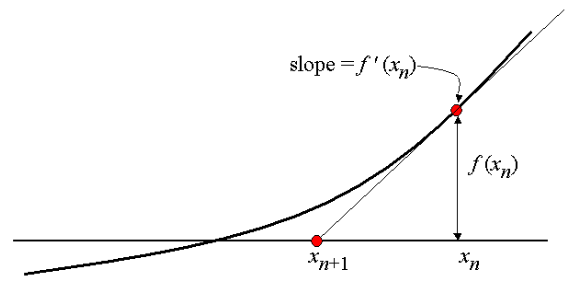
\includegraphics[width=10cm]{images/Newton_Geo.png}
        \end{center}
        \caption{Biểu diễn hình học phương pháp Newton-Raphson}
\end{figure}\\
\hspace*{0.5cm} {Ta vẽ một đường tiếp tuyến với đồ thị $f(x)$ tại điểm $x=x_n$. Đường thẳng này có hệ số góc $f'(x_n)$ và đi qua điểm $(x_n, f(x_n)$ nên có phương trình $y = f'(x_n)(x - x_n) + f(x_n)$. Bây giờ ta tìm nghiệm xấp xỉ mới $x_{n+1}$ của phương trình này. Giải phương trình ta được $x_{n+1} = x_n - \frac{f(x_n)}{f'(x_n)}$}.
\hspace*{0.5cm} {Tuy nhiên phương pháp Newton - Raphson cũng có những giới hạn nhất định. Phương pháp này có thể không hoạt động nếu có các điểm uốn, điểm cực đại hoặc cực tiểu địa phương xung quanh điểm làm gốc $x_0$.}\\
\hspace*{0.5cm} {Phương pháp Newton - Raphson cũng có thể được mở rộng cho hệ phương trình. Cụ thể, đối với hệ phương trình vi phân tổng quát của bài tập này, công thức hồi quy của phương pháp Newton - Raphson sẽ có dạng:}\\
\centerline{$\begin{bmatrix}
    R_{new} \\
    J_{new}
\end{bmatrix} = \begin{bmatrix}
    R_{old} \\
    J_{old}
\end{bmatrix} - \alpha.\begin{bmatrix}
    \frac{\partial f}{\partial R} & \frac{\partial f}{\partial J}\\
    \frac{\partial g}{\partial R} & \frac{\partial g}{\partial J}
\end{bmatrix}^{-1}\begin{bmatrix}
    f \\
    g
\end{bmatrix}$}\\
Trong công thức trên:
\begin{itemize}
    \item $\begin{bmatrix}
    R_{new} \\
    J_{new}
    \end{bmatrix}$ là các giá trị xấp xỉ mới.
    \item $\begin{bmatrix}
    R_{new} \\
    J_{new}
    \end{bmatrix}$ là các giá trị cũ.
    \item $\begin{bmatrix}
    \frac{\partial f}{\partial R} & \frac{\partial f}{\partial J}\\
    \frac{\partial g}{\partial R} & \frac{\partial g}{\partial J}
    \end{bmatrix}$ là ma trận Jacobian: Ma trận Jacobian là ma trận chứa các đạo hàm riêng bậc nhất của các hàm $f, g$ theo các biến $R, J$.
    \item $\begin{bmatrix}
    f \\
    g
    \end{bmatrix}$ là các hàm $f, g$ trong hệ phương trình vi phân.
    \item $\alpha$ là một hệ số chọn. Trong 5 ví dụ bên dưới, ta chọn $\alpha = 1$. 
\end{itemize}
\hspace*{0.5cm}{Giá trị đầu vào cho công thức hồi quy phải ở dạng phương trình Euler ẩn, với các biến, các hàm được định nghĩa như phía dưới:}
\begin{align*}
    R_{k+1} = R_k + f(t_{k+1}, R_{k+1}, J_{k+1}) * h\\
    J_{k+1} = J_k + g(t_{k+1}, R_{k+1}, J_{k+1}) * h
\end{align*}
\hspace*{0.5cm}{Ta đưa hai phương trình trên về dạng sau để áp dụng giải thuật Newton - Raphson:}
\begin{align*}
    R_k + f(t_{k+1}, R_{k+1}, J_{k+1}) * h - R_{k+1} = 0\\
    J_k + g(t_{k+1}, R_{k+1}, J_{k+1}) * h - J{k+1} = 0
\end{align*}
\subsubsection{Nguồn gốc}
\hspace*{0.5cm} {Lấy tích phân phương trình vi phân từ $t_k$ tới $t_k + h$ và áp dụng các định lí cơ bản của tích phân và vi phân để có được:}\\
\hspace*{4cm} {$R(t_k + h) - R(t_k) = \displaystyle\int\limits_{t_k}^{t_k + h}f(
t, R(t), J(t)\;\mathrm{d}t$}\\
\hspace*{0.5cm} {Tính xấp xỉ tích phân trên bằng tổng Riemann phải, ta được:}\\
\hspace*{4cm} {$\displaystyle\int\limits_{t_k}^{t_k + h}f(t, R(t), J(t)\;\mathrm{d}t \approx hf(t_{k+1}, R(t_{k+1}), J(t_{k+1})$}\\
\hspace*{0.5cm} {Kết hợp cả 2 phương trình, ta suy ra phương pháp Euler ẩn. Chứng minh tương tự với hàm $J(t)$.}
\subsubsection{Sai số cắt ngắn cục bộ}
\hspace*{0.5cm} {Giống với phương pháp Euler tường minh, sai số cắt ngắn cục bộ của phương pháp Euler ẩn cũng được tính theo công thức:}\\
\hspace*{4cm} {$E(t_1) = \sqrt{[R(t_1) - R_1]^2 + [J(t_1) - J_1]^2}$}\\
\hspace*{0.5cm} {Với $t_0 = t_1 - h$, áp dụng khai triển Taylor đối với $R(t_0)$ và $J(t_0)$, ta có:}
\begin{align}
    \begin{cases}
        R(t_0) = R(t_1 - h) = R(t_1) - h.R'(t_1) + \frac{1}{2}h^2R"(t_1) + O(h^2)\\
        J(t_0) = J(t_1 - h) = J(t_1) - h.J'(t_1) + \frac{1}{2}h^2J"(t_1) + O(h^2)
    \end{cases}
\end{align}
\begin{align}
    \Rightarrow
    \begin{cases}
        R_0 = R(t_1) - h.f(t_1, R_1, J_1) + \frac{1}{2}h^2f'(t_1, R_1, J_1) + O(h^2)\\
        J_0 = J(t_1) - h.g(t_1, R_1, J_1) + \frac{1}{2}h^2g'(t_1, R_1, J_1) + O(h^2)
    \end{cases}
\end{align}
\begin{align}
    \Rightarrow
    \begin{cases}
        R(t_1) = R_1 - \frac{1}{2}h^2f'(t_1, R_1, J_1) + O(h^2)\\
        J(t_1) = J_1 - \frac{1}{2}h^2g'(t_1, R_1, J_1) + O(h^2)
    \end{cases}
\end{align}
\begin{align}
    \Rightarrow
    \begin{cases}
        R(t_1) - R_1 = -\frac{1}{2}h^2f'(t_1, R_1, J_1) + O(h^2)\\
        J(t_1) - J_1 = -\frac{1}{2}h^2g'(t_1, R_1, J_1) + O(h^2)
    \end{cases}
\end{align}
\hspace*{0.5cm} {Bỏ qua phần $O(h^2)$ ta được:}
\begin{align}
    \begin{cases}
        R(t_1) - R_1 = -\frac{1}{2}h^2f'(t_1, R_1, J_1)\\
        J(t_1) - J_1 = -\frac{1}{2}h^2g'(t_1, R_1, J_1)
    \end{cases}
\end{align}
\hspace*{3cm} {$\Rightarrow E(t_1) \approx \sqrt{[-\frac{1}{2}h^2f'(t_1, R_1, J_1)]^2 + [-\frac{1}{2}h^2g'(t_1, R_1, J_1)]^2}$}\\
\hspace*{4cm} {$= \frac{1}{2}h^2\sqrt{f'^2(t_1,R_1,J_1) + g'^2(t_1,R_1,J_1)}$}\\
\hspace*{0.5cm} {Như vậy, trong phương pháp Euler ẩn, $E(t_1)$ cũng xấp xỉ tỉ lệ thuận với $h^2$.}
\subsubsection{Nhược điểm của phương pháp Euler ẩn}
\hspace*{0.5cm} {Thứ nhất, do trong công thức của phương pháp Euler ẩn có ẩn số $R_{k+1}$ và $J_{k+1}$ ở cả 2 vế của hệ phương trình, nên để tìm được chúng, ta phải giải hệ phương trình đó. Quá trình này có thể tốn nhiều thời gian và phức tạp hơn so với phương pháp Euler tường minh.}\\
\hspace*{0.5cm} {Thứ hai, sai số cắt ngắn cục bộ tỉ lệ thuận với $h^2$, điều này đồng nghĩa với việc khi $h > 1$ sai số sẽ trở nên rất lớn, khi đó khoảng cách giữa nghiệm chính xác và nghiệm gần đúng sẽ là rất lớn, ảnh hưởng tới tính đúng đắn của bài toán}
\subsubsection{Ví dụ}
\textbf{Ví dụ 1:} Tìm nghiệm xấp xỉ của hệ phương trình bằng phương pháp Euler ẩn:
\begin{align*}
    \begin{cases}
        R'=-R+J+\frac{sin(t+1)}{t+1}\\
        J'=-R+J+t \\
        R(0)=2, J(0)=3
    \end{cases}
\end{align*}
\centerline{\textbf{Giải}}\\
Đây là ví dụ về hệ phương trình vi phân tuyến tính không thuần nhất không thể tìm nghiệm chính xác với điều kiện ban đầu $R_0=2, J_0=3$.\\
Công thức hồi quy như sau:
\begin{align*}
    \begin{cases}
        R_n=R_{n-1}+h(-R_n+J_n+\frac{sin(t_n+1)}{t_n+1})\\
        J_n=J_{n-1}+h(-R_n+J_n+t_n)\\
        t_n=t_{n-1}+h
    \end{cases}
\end{align*}
\begin{enumerate}
    \item \textbf{Vẽ đồ thị nghiệm.}\\
    Biểu diễn $R$ và $J$ trên cùng một đồ thị theo biến thời gian $t$ (hình 25):
    \begin{figure}[h!]
        \begin{center}
        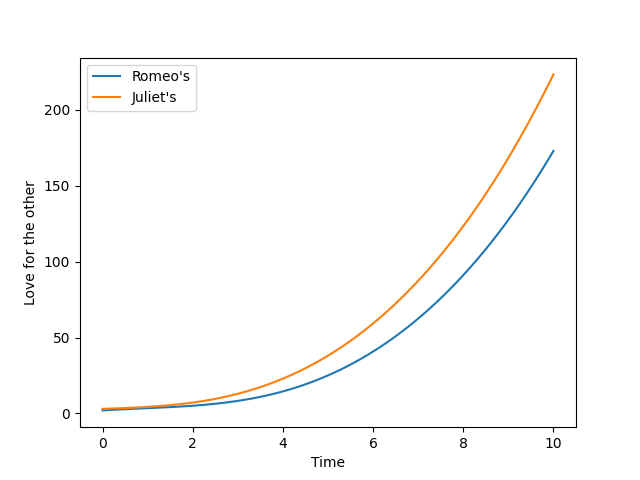
\includegraphics[width=10cm]{images/euler_1.png}
        \end{center}
        \caption{Solution figure Ví dụ 1}
    \end{figure}\\
    Giải thích các đoạn code trong Python vẽ đồ thị ví dụ trên (các đoạn code này được ta định nghĩa trong file \textbf{implicit\_euler\_trajectory.py} và sẽ được dùng để vẽ \textbf{phase portrait}) như sau:
    \begin{itemize}
        \item Nạp các modules cần thiết, bao gồm: \textbf{matplotlib.pyplot}(module đồ họa vẽ đồ thị), \textbf{numpy}(module toán học xử lý ma trận và mảng), \textbf{numpy.linalg.inv}(module để nghịch đảo ma trận), \textbf{math}(hình 26).
        \begin{figure}[h!]
            \begin{center}
            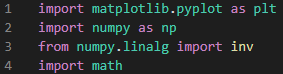
\includegraphics[width=5cm]{images/euler_modules.png}
            \end{center}
            \caption{Nạp modules}
        \end{figure}
        \item Tạo 3 công thức của phương pháp Euler ẩn dưới dạng \textbf{Newton-Raphson} tương ứng với $R$ (Romeo), $J$ (Juliet), $t$ (Thời điểm) (Ở đây, ta tạo thêm một công thức Euler ẩn so với kiến thức chuẩn bị cho biến thời gian $t$ với \textbf{time step = h})(hình 27):
        \begin{center}
            \textbf{\textit{old\_value + h * f(new\_value) - new\_value}}
        \end{center}
         \begin{figure}[h!]
            \begin{center}
            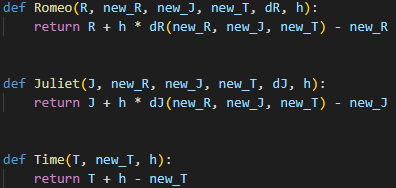
\includegraphics[width=8cm]{images/euler_func.png}
            \end{center}
            \caption{Công thức Euler ẩn của \textbf{Romeo, Juliet, Time}}
        \end{figure}
        \item Tạo ma trận \textbf{Jacobian} để tính toán đạo hàm riêng theo từng biến của 3 công thức Euler ẩn của hệ phương trình vi phân đa biến (Ma trận \textbf{Jacobian} bao gồm 9 hạng tử) (hình 28).
         \begin{figure}[h!]
            \begin{center}
            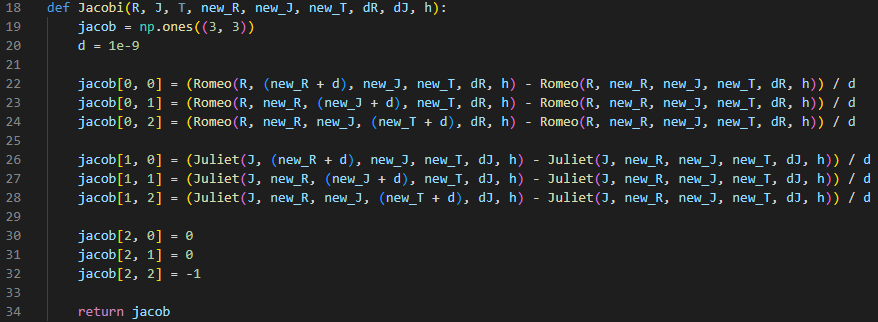
\includegraphics[width=12cm]{images/jacobi.png}
            \end{center}
            \caption{Ma trận Jacobian}
        \end{figure}
        \item Viết thuật toán \textbf{Newton-Raphson}, vòng lặp của thuật toán \textbf{Newton-Raphson} dừng lại khi sai số cắt ngắn cục bộ \textbf{LTE} có thể chấp nhận được (cụ thể $error < 10^{-9}$) tại một thời điểm $t$ (hình 29).
         \begin{figure}[h!]
            \begin{center}
            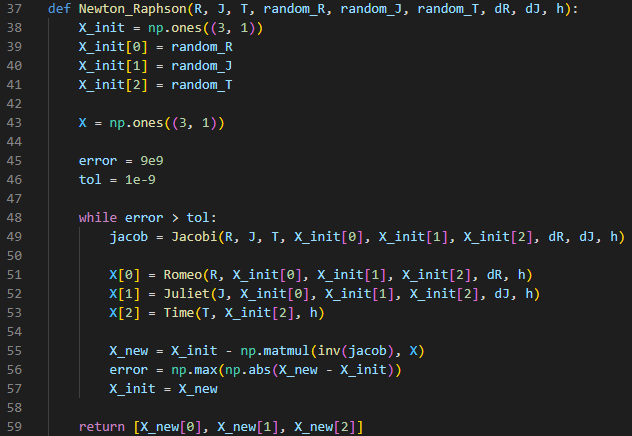
\includegraphics[width=10cm]{images/Newton_Raphson.png}
            \end{center}
            \caption{Giải thuật \textbf{Newton-Raphson}}
        \end{figure}
        \item Viết hàm \textbf{implicit\_euler} theo phương pháp Euler ẩn sử dụng giải thuật \textbf{Newton-Raphson} để tính toán nghiệm xấp xỉ cho hệ phương trình vi phân (hình 30).
         \begin{figure}[h!]
            \begin{center}
            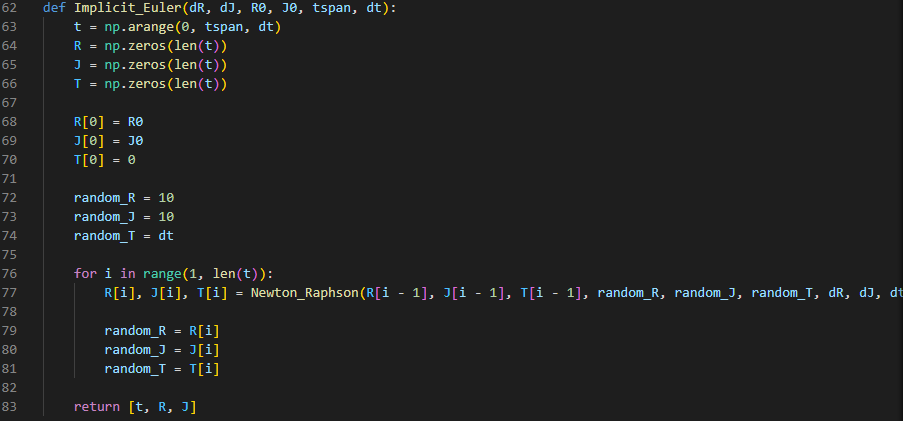
\includegraphics[width=14cm]{images/implicit_euler.png}
            \end{center}
            \caption{Phương pháp Euler ẩn}
        \end{figure}
        \item Cuối cùng ta nhập các công thức của $R', J'$, các giá trị ban đầu $R_0, J_0$ đã cho trong hệ phương trình vi phân. Chọn bước nhảy thời gian \textbf{time step} $h = 0.001$ và sau đó vẽ hình (hình 31).
        \begin{figure}[h!]
            \begin{center}
            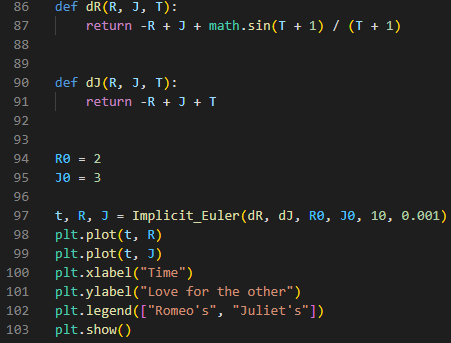
\includegraphics[width=8cm]{images/euler_plot.png}
            \end{center}
            \caption{Nhập input và xuất ra output}
        \end{figure}
    \end{itemize}
    \item \textbf{Vẽ Phase portrait}\\
    Phase portrait của hệ phương trình vi phân
    \begin{align*}
        \begin{cases}
            R'=-R+J+\frac{sin(t+1)}{t+1}\\
            J'=-R+J+t
        \end{cases}
    \end{align*}
    với điều kiện ban đầu bất kì trong mặt phẳng $RJ$ được biểu diễn trong hình 32.
    \begin{figure}[h!]
        \begin{center}
        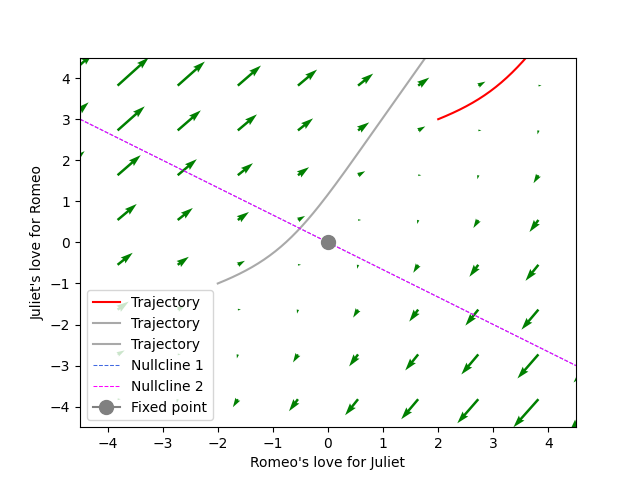
\includegraphics[width=10cm]{images/euler_1_portrait.png}
        \end{center}
        \caption{Phase portrait figure}
    \end{figure}\\
    Đoạn code Python được sử dụng để vẽ phase portrait tương tự như \textbf{Bài tập 2}:
    \begin{lstlisting}
        import numpy as np
        import matplotlib.pyplot as plt
        from scipy.integrate import odeint
        from implicit_euler_trajectory import dR, dJ, R0, J0
        Sts = [[R0, J0], [R0 + 4, J0 + 4], [R0 - 4, J0 - 4]]
        # ODE System
        
        
        def ivpSys(s, t, dR, dJ):
            R, J = s
            T = t
            dRdt = dR(R, J, T)
            dJdt = dJ(R, J, T)
            return [dRdt, dJdt]
        
        
        # Vector R', J' at t = 0 with 144 values of pair (R0, J0)
        y1 = np.linspace(-6, 6, 12)
        y2 = np.linspace(-6, 6, 12)
        Y1, Y2 = np.meshgrid(y1, y2)
        t = 0
        u, v = np.zeros(Y1.shape), np.zeros(Y2.shape)
        NI, NJ = Y1.shape
        for i in range(NI):
            for j in range(NJ):
                x = Y1[i, j]
                y = Y2[i, j]
                yvector = ivpSys([x, y], t, dR, dJ)
                u[i, j] = yvector[0]
                v[i, j] = yvector[1]
        Q = plt.quiver(Y1, Y2, u, v, color='g')
        # Trajectory of Sts with 200 values of t between (0,5)
        tspan = np.linspace(0, 5, 200)
        for elementSt, St in enumerate(Sts):
            sol = odeint(ivpSys, St, tspan, args=(dR, dJ))
            if elementSt == 0:
                color = "r"
            else:
                color = "darkgray"
            plt.plot(sol[:, 0], sol[:, 1], color, label='Trajectory')
        # Figure phase portrait
        x = np.linspace(-4.5, 4.5, 100)
        
        
        def fx(x, a, b):
            return -a * x / b
        
        
        plt.plot(x, fx(x, 2, 3), linestyle='dashed', linewidth=0.75,
                 color='royalblue', label='Nullcline 1')
        plt.plot(x, fx(x, 2, 3), linestyle='dashed', linewidth=0.75,
                 color='magenta', label='Nullcline 2')
        plt.plot(0, 0, "red", marker="o", markersize=10.0,
                 color='grey', label='Fixed point')
        plt.xlabel("Romeo's love for Juliet")
        plt.ylabel("Juliet's love for Romeo")
        plt.legend()
        plt.xlim([-4.5, 4.5])
        plt.ylim([-4.5, 4.5])
        plt.show()
    \end{lstlisting}
\end{enumerate}
\textbf{Ví dụ 2:}  Tìm nghiệm xấp xỉ của hệ phương trình bằng phương pháp Euler ẩn:
\begin{align*}
    \begin{cases}
        R'=R(1 - J) \\
        J'=R(1 - J) \\
        R(0)=2, J(0)=3
    \end{cases}
\end{align*}
\centerline{\textbf{Giải}}\\
Đây là ví dụ về hệ phương trình vi phân thường cấp 1 tổng quát không thể tìm nghiệm chính xác với điều kiện ban đầu $R0=2, J0=3$.\\
Công thức hồi quy như sau:
\begin{align*}
    \begin{cases}
        R_n=R_{n-1}+h(R_n - R_n * J_n)\\
        J_n=J_{n-1}+h(R_n - R_n * J_n)\\
        T_n=T_{n-1}+h
    \end{cases}
\end{align*}
Chọn $h=0.001$. Đoạn code trong Python dùng để vẽ đồ thị và phase portrait tương tự như \textbf{ví dụ 1}, chỉ thay đổi $dR, dJ, R0, J0$. Hình vẽ được biểu diễn ở hình 33.
\begin{figure}[h!]
    \begin{center}
        \begin{tabular}{cc}
             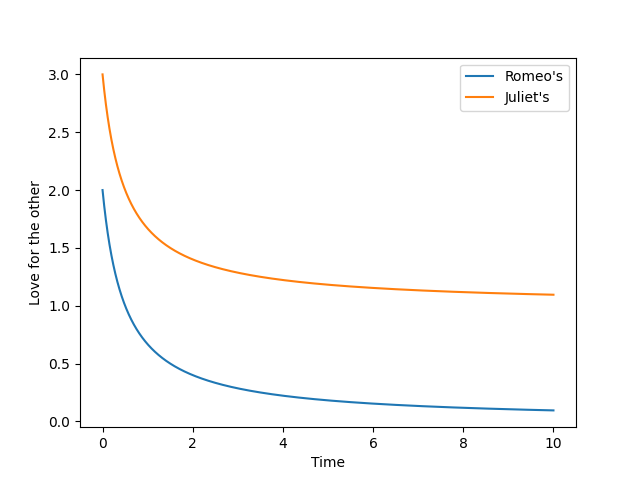
\includegraphics[width=7cm]{images/euler_2.png} &
             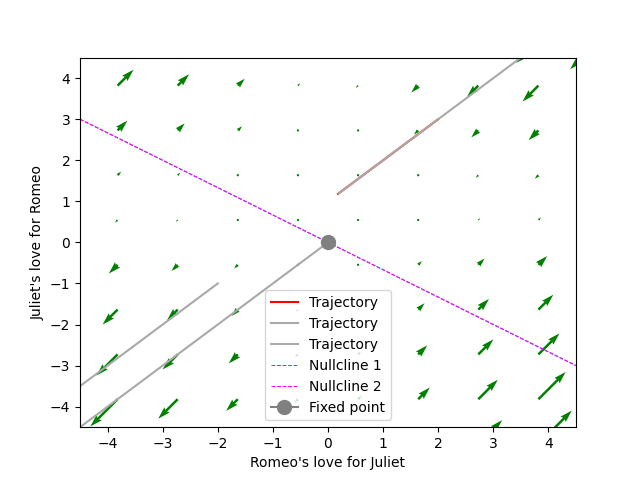
\includegraphics[width=7cm]{images/euler_2_portrait.png}\\
        \end{tabular}
        \caption{Solution figure và phase portrait figure Ví dụ 2}
    \end{center}
\end{figure}\\
\textbf{Ví dụ 3:}  Tìm nghiệm xấp xỉ của hệ phương trình bằng phương pháp Euler ẩn:
\begin{align*}
    \begin{cases}
        R'=-3R+4J+sin(t)\\
        J'=-2R+3J+t\\
        R(0)=0, J(0)=1
    \end{cases}
\end{align*}
\centerline{\textbf{Giải}}\\
Đây là ví dụ về hệ phương trình vi phân tuyến tính không thuần nhất với hệ số không đổi và giá trị ban đầu $R0 = 0, J0 = 1$.\\
Công thức hồi quy như sau:
\begin{align*}
    \begin{cases}
        R_n=R_{n-1}+h(-3R_n+4J_n+\sin(T_n))\\
        J_n=J_{n-1}+h(-2R_n+3J_n+T_n)\\
        T_n=T_{n-1}+h
    \end{cases}
\end{align*}
Chọn $h=0.001$. Đoạn code trong Python dùng để vẽ đồ thị và phase portrait tương tự như \textbf{ví dụ 1}, chỉ thay đổi $dR, dJ, R0, J0$. Hình vẽ được biểu diễn ở hình 34.
\begin{figure}[h!]
    \begin{center}
        \begin{tabular}{cc}
             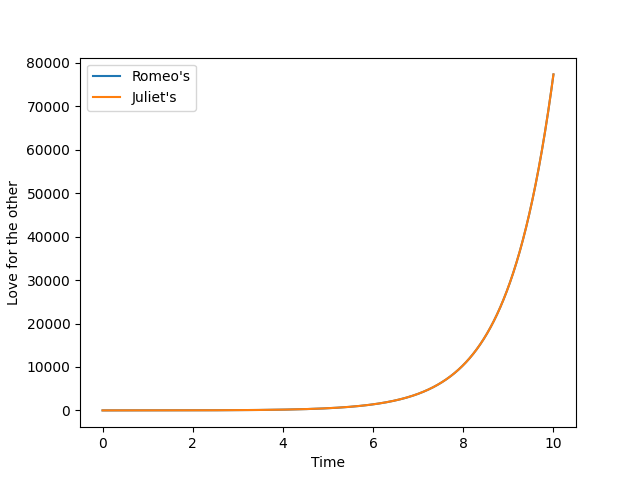
\includegraphics[width=7cm]{images/euler_3.png} &
             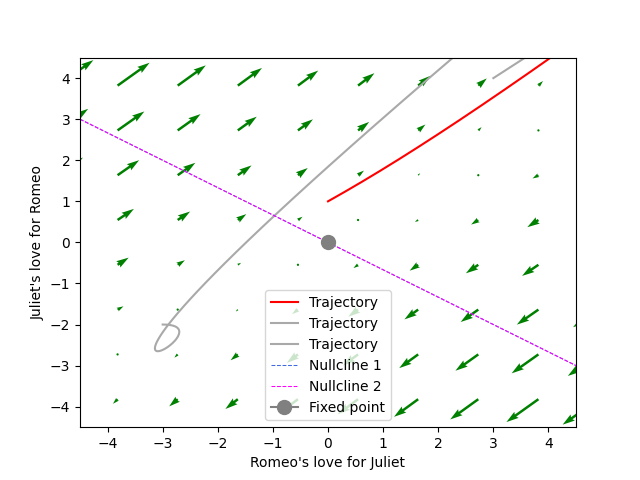
\includegraphics[width=7cm]{images/euler_3_portrait.png}\\
        \end{tabular}
        \caption{Solution figure và phase portrait figure Ví dụ 3}
    \end{center}
\end{figure}\\
\textbf{Ví dụ 4:}  Tìm nghiệm xấp xỉ của hệ phương trình bằng phương pháp Euler ẩn:
\begin{align*}
    \begin{cases}
        R'=J+t-1\\
        J'=-R+t^2\\
        R(0)=1, J(0)=2
    \end{cases}
\end{align*}
\centerline{\textbf{Giải}}\\
Đây là ví dụ về hệ phương trình vi phân tuyến tính không thuần nhất với hệ số không đổi và giá trị ban đầu $R0 = 1, J0 = 2$.\\
Công thức hồi quy như sau:
\begin{align*}
    \begin{cases}
        R_n=R_{n-1}+h(J_n + T_n - 1)\\
        J_n=J_{n-1}+h(-R_n + T_n^2)\\
        T_n=T_{n-1}+h
    \end{cases}
\end{align*}
Chọn $h=0.001$. Đoạn code trong Python dùng để vẽ đồ thị và phase portrait tương tự như \textbf{ví dụ 1}, chỉ thay đổi $dR, dJ, R0, J0$. Hình vẽ được biểu diễn ở hình 35.
\begin{figure}[h!]
    \begin{center}
        \begin{tabular}{cc}
             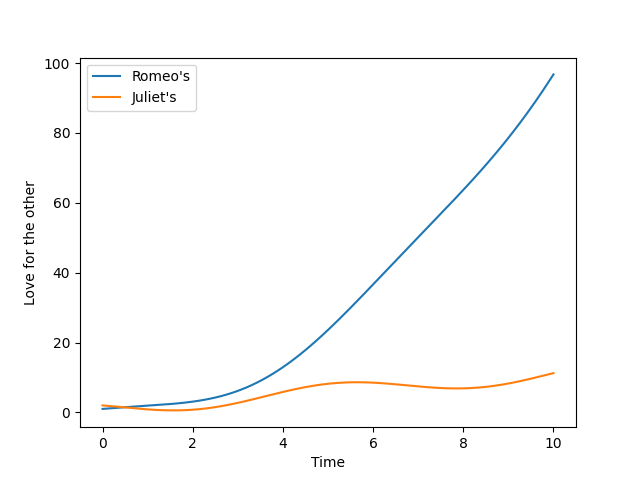
\includegraphics[width=7cm]{images/euler_4.png} &
             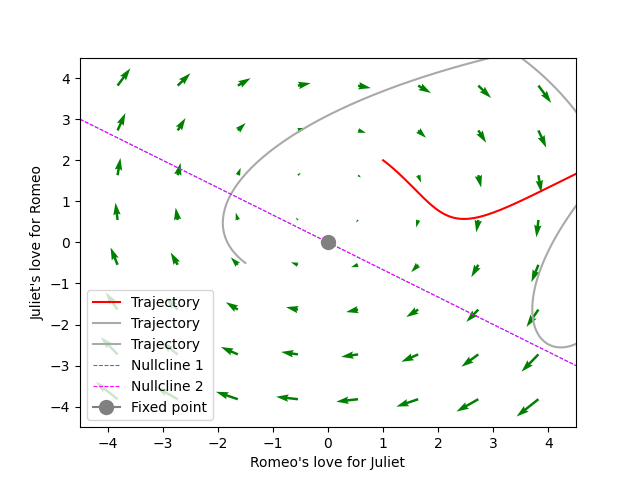
\includegraphics[width=7cm]{images/euler_4_portrait.png}\\
        \end{tabular}
        \caption{Solution figure và phase portrait figure Ví dụ 4}
    \end{center}
\end{figure}\\
\textbf{Ví dụ 5:}  Tìm nghiệm xấp xỉ của hệ phương trình bằng phương pháp Euler ẩn:
\begin{align*}
    \begin{cases}
        R'=-4R + RJ\\
        J'=R^2 - 3J\\
        R(0)=2, J(0)=3
    \end{cases}
\end{align*}
\centerline{\textbf{Giải}}\\
Đây là ví dụ về hệ phương trình vi phân thường cấp 1 tổng quát không thể tìm nghiệm chính xác với điều kiện ban đầu $R0 = 2, J0 = 3$.\\
Công thức hồi quy như sau:
\begin{align*}
    \begin{cases}
        R_n=R_{n-1}+h(-4R_n + R_nJ_n)\\
        J_n=J_{n-1}+h(R_n^2 - 3J_n)\\
        T_n=T_{n-1}+h
    \end{cases}
\end{align*}
Chọn $h=0.001$. Đoạn code trong Python dùng để vẽ đồ thị và phase portrait tương tự như \textbf{ví dụ 1}, chỉ thay đổi $dR, dJ, R0, J0$. Hình vẽ được biểu diễn ở hình 36.
\begin{figure}[h!]
    \begin{center}
        \begin{tabular}{cc}
             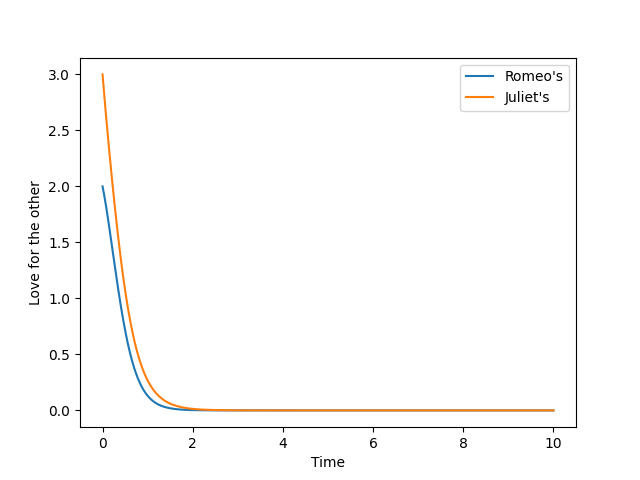
\includegraphics[width=7cm]{images/euler_5.png} &
             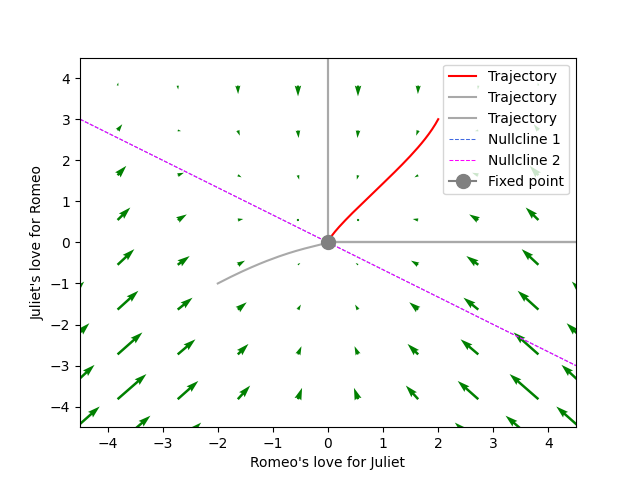
\includegraphics[width=7cm]{images/euler_5_portrait.png}\\
        \end{tabular}
        \caption{Solution figure và phase portrait figure Ví dụ 5}
    \end{center}
\end{figure}\\
\textbf{Link toàn bộ bài làm của nhóm:}\\
\url{https://github.com/ngyngcphu/Dynamics-of-Love}
\newpage
\addcontentsline{toc}{section}{Tài liệu tham khảo}
\begin{thebibliography}{99999}
\bibitem[1]{1}{Vladimir I Arnold.} {\em Ordinary Differential Equations.}  Springer Science \& Business Media, 1992.

\bibitem[2]{2}{Morris W Hirsch and Stephen Smale.} {\em Differential Equations, Dynamical Systems, and Linear Algebra.} Academic Press, 1974.

\bibitem[3]{3}{David G Luenberger.} {\em Introduction to Dynamic Systems: Theory, Models, and Applications,} volume 1. Wiley New York, 1979.

\bibitem[4]{4}{Steven H Strogatz.}{  Love affairs and differential equations.} {\em Mathematics Magazine,} 61(1):35–35, 1988.

\bibitem[5]{5}{Phương trình vi phân - Phương pháp giá trị riêng giải hệ phương trình vi phân tuyến thuần nhất}\\
\url{https://www.youtube.com/watch?v=LVbsb6mAFZ4}

\bibitem[6]{6}{Phase portraits.}\\
\url{https://www.math.colostate.edu/~gerhard/M345/CHP/ch9_3-4.pdf}

\bibitem[7]{7}{Giải thuật Newton-Rahpson}\\
\url{https://brilliant.org/wiki/newton-raphson-method/}

\bibitem[8]{8}{Phương pháp Implicit-Euler}\\
\url{https://skill-lync.com/student-projects/Solving-a-system-of-ODEs-using-Implicit-Euler-method-86502}
\end{thebibliography}
\end{document}

